% Options for packages loaded elsewhere
\PassOptionsToPackage{unicode}{hyperref}
\PassOptionsToPackage{hyphens}{url}
%
\documentclass[
]{article}
\usepackage{lmodern}
\usepackage{amssymb,amsmath}
\usepackage{ifxetex,ifluatex}
\ifnum 0\ifxetex 1\fi\ifluatex 1\fi=0 % if pdftex
  \usepackage[T1]{fontenc}
  \usepackage[utf8]{inputenc}
  \usepackage{textcomp} % provide euro and other symbols
\else % if luatex or xetex
  \usepackage{unicode-math}
  \defaultfontfeatures{Scale=MatchLowercase}
  \defaultfontfeatures[\rmfamily]{Ligatures=TeX,Scale=1}
\fi
% Use upquote if available, for straight quotes in verbatim environments
\IfFileExists{upquote.sty}{\usepackage{upquote}}{}
\IfFileExists{microtype.sty}{% use microtype if available
  \usepackage[]{microtype}
  \UseMicrotypeSet[protrusion]{basicmath} % disable protrusion for tt fonts
}{}
\makeatletter
\@ifundefined{KOMAClassName}{% if non-KOMA class
  \IfFileExists{parskip.sty}{%
    \usepackage{parskip}
  }{% else
    \setlength{\parindent}{0pt}
    \setlength{\parskip}{6pt plus 2pt minus 1pt}}
}{% if KOMA class
  \KOMAoptions{parskip=half}}
\makeatother
\usepackage{xcolor}
\IfFileExists{xurl.sty}{\usepackage{xurl}}{} % add URL line breaks if available
\IfFileExists{bookmark.sty}{\usepackage{bookmark}}{\usepackage{hyperref}}
\hypersetup{
  pdftitle={EDA},
  pdfauthor={Ignacio Vellido},
  hidelinks,
  pdfcreator={LaTeX via pandoc}}
\urlstyle{same} % disable monospaced font for URLs
\usepackage[margin=1in]{geometry}
\usepackage{color}
\usepackage{fancyvrb}
\newcommand{\VerbBar}{|}
\newcommand{\VERB}{\Verb[commandchars=\\\{\}]}
\DefineVerbatimEnvironment{Highlighting}{Verbatim}{commandchars=\\\{\}}
% Add ',fontsize=\small' for more characters per line
\usepackage{framed}
\definecolor{shadecolor}{RGB}{248,248,248}
\newenvironment{Shaded}{\begin{snugshade}}{\end{snugshade}}
\newcommand{\AlertTok}[1]{\textcolor[rgb]{0.94,0.16,0.16}{#1}}
\newcommand{\AnnotationTok}[1]{\textcolor[rgb]{0.56,0.35,0.01}{\textbf{\textit{#1}}}}
\newcommand{\AttributeTok}[1]{\textcolor[rgb]{0.77,0.63,0.00}{#1}}
\newcommand{\BaseNTok}[1]{\textcolor[rgb]{0.00,0.00,0.81}{#1}}
\newcommand{\BuiltInTok}[1]{#1}
\newcommand{\CharTok}[1]{\textcolor[rgb]{0.31,0.60,0.02}{#1}}
\newcommand{\CommentTok}[1]{\textcolor[rgb]{0.56,0.35,0.01}{\textit{#1}}}
\newcommand{\CommentVarTok}[1]{\textcolor[rgb]{0.56,0.35,0.01}{\textbf{\textit{#1}}}}
\newcommand{\ConstantTok}[1]{\textcolor[rgb]{0.00,0.00,0.00}{#1}}
\newcommand{\ControlFlowTok}[1]{\textcolor[rgb]{0.13,0.29,0.53}{\textbf{#1}}}
\newcommand{\DataTypeTok}[1]{\textcolor[rgb]{0.13,0.29,0.53}{#1}}
\newcommand{\DecValTok}[1]{\textcolor[rgb]{0.00,0.00,0.81}{#1}}
\newcommand{\DocumentationTok}[1]{\textcolor[rgb]{0.56,0.35,0.01}{\textbf{\textit{#1}}}}
\newcommand{\ErrorTok}[1]{\textcolor[rgb]{0.64,0.00,0.00}{\textbf{#1}}}
\newcommand{\ExtensionTok}[1]{#1}
\newcommand{\FloatTok}[1]{\textcolor[rgb]{0.00,0.00,0.81}{#1}}
\newcommand{\FunctionTok}[1]{\textcolor[rgb]{0.00,0.00,0.00}{#1}}
\newcommand{\ImportTok}[1]{#1}
\newcommand{\InformationTok}[1]{\textcolor[rgb]{0.56,0.35,0.01}{\textbf{\textit{#1}}}}
\newcommand{\KeywordTok}[1]{\textcolor[rgb]{0.13,0.29,0.53}{\textbf{#1}}}
\newcommand{\NormalTok}[1]{#1}
\newcommand{\OperatorTok}[1]{\textcolor[rgb]{0.81,0.36,0.00}{\textbf{#1}}}
\newcommand{\OtherTok}[1]{\textcolor[rgb]{0.56,0.35,0.01}{#1}}
\newcommand{\PreprocessorTok}[1]{\textcolor[rgb]{0.56,0.35,0.01}{\textit{#1}}}
\newcommand{\RegionMarkerTok}[1]{#1}
\newcommand{\SpecialCharTok}[1]{\textcolor[rgb]{0.00,0.00,0.00}{#1}}
\newcommand{\SpecialStringTok}[1]{\textcolor[rgb]{0.31,0.60,0.02}{#1}}
\newcommand{\StringTok}[1]{\textcolor[rgb]{0.31,0.60,0.02}{#1}}
\newcommand{\VariableTok}[1]{\textcolor[rgb]{0.00,0.00,0.00}{#1}}
\newcommand{\VerbatimStringTok}[1]{\textcolor[rgb]{0.31,0.60,0.02}{#1}}
\newcommand{\WarningTok}[1]{\textcolor[rgb]{0.56,0.35,0.01}{\textbf{\textit{#1}}}}
\usepackage{graphicx,grffile}
\makeatletter
\def\maxwidth{\ifdim\Gin@nat@width>\linewidth\linewidth\else\Gin@nat@width\fi}
\def\maxheight{\ifdim\Gin@nat@height>\textheight\textheight\else\Gin@nat@height\fi}
\makeatother
% Scale images if necessary, so that they will not overflow the page
% margins by default, and it is still possible to overwrite the defaults
% using explicit options in \includegraphics[width, height, ...]{}
\setkeys{Gin}{width=\maxwidth,height=\maxheight,keepaspectratio}
% Set default figure placement to htbp
\makeatletter
\def\fps@figure{htbp}
\makeatother
\setlength{\emergencystretch}{3em} % prevent overfull lines
\providecommand{\tightlist}{%
  \setlength{\itemsep}{0pt}\setlength{\parskip}{0pt}}
\setcounter{secnumdepth}{-\maxdimen} % remove section numbering
\usepackage{booktabs}
\usepackage{longtable}
\usepackage{array}
\usepackage{multirow}
\usepackage{wrapfig}
\usepackage{float}
\usepackage{colortbl}
\usepackage{pdflscape}
\usepackage{tabu}
\usepackage{threeparttable}
\usepackage{threeparttablex}
\usepackage[normalem]{ulem}
\usepackage{makecell}
\usepackage{xcolor}

\title{EDA}
\author{Ignacio Vellido}
\date{11/13/2020}

\begin{document}
\maketitle

\hypertarget{intro}{%
\section{Intro}\label{intro}}

Para este trabajo contamos con dos datasets distintos:
\textbf{habermanMPG6} para aplicar Regresión y \textbf{haberman} para
aplicar Clasificación.

\hypertarget{descripciones-de-los-problemas}{%
\subsection{Descripciones de los
problemas}\label{descripciones-de-los-problemas}}

\hypertarget{haberman}{%
\subsubsection{haberman}\label{haberman}}

\url{http://archive.ics.uci.edu/ml/datasets/Haberman\%27s+Survival}
\url{https://sci2s.ugr.es/keel/dataset.php?cod=62}

Este dataset codifica el ratio de supervivencia de pacientes operados de
cáncer de pecho en el Hospital Universitario de Chicago, en base a las
siguientes características:

\begin{enumerate}
\def\labelenumi{\arabic{enumi}.}
\tightlist
\item
  Age: Indica la edad del paciente en el momento de la operación.
\item
  Year: Los dos últimas cifras del año en el que se operó el paciente.
\item
  Positive: Número de nodos auxiliares positivos detectados. Esta
  variable hace referencia a los ganglios linfáticos que dan positivos
  como presentes de cáncer. A mayor número de nodos detectados, mayor es
  la gravedad del cáncer. Aunque normalmente la primera zona de
  propagación del cáncer son estos nodos, no es la única medida de la
  seriedad, pues este puede propagarse a otras zonas del cuerpo. En
  principio deberíamos suponer la posibilidad de que puede haber cosas
  de no supervivencia con bajo número de positivos, pero la bibliografía
  nos asegura que la probabilidad es baja.
\end{enumerate}

Viendo que solo tenemos esta medida del cáncer en el dataset es posible
que la operación que recibieron los pacientes sea algún tipo de cirugía
de ganglios linfáticos, donde el cirujano intenta extraer los nodos
afectados por el tumor. Por consiguiente, cuanto mayor es la cantidad de
nodos detectados, más complicaciones pueden acarrearse de la operación.
(poner referencias)

\url{https://www.cancer.org/cancer/breast-cancer/treatment/surgery-for-breast-cancer/lymph-node-surgery-for-breast-cancer.html}
\url{https://en.wikipedia.org/wiki/Lymph_node\#}:\textasciitilde:text=A\%20lymph\%20node\%2C\%20or\%20lymph,include\%20B\%20and\%20T\%20cells.

El objetivo es poder clasificar, en base a los tres atributos, si los
pacientes pueden sobrevir 5 años o más:

\begin{enumerate}
\def\labelenumi{\arabic{enumi}.}
\setcounter{enumi}{3}
\tightlist
\item
  Survival: Sí/No indicando la supervivencia del paciente tras 5 años.
\end{enumerate}

BUSCAR POSIBLES COMPLICACIONES

Contamos por tanto con un problema de clasificación binario en base a
tres características, y con un número total de 306 instancias.

\begin{center}\rule{0.5\linewidth}{0.5pt}\end{center}

\hypertarget{anuxe1lisis-estaduxedstico-de-datos}{%
\section{Análisis Estadístico de
Datos}\label{anuxe1lisis-estaduxedstico-de-datos}}

\hypertarget{haberman-1}{%
\subsubsection{haberman}\label{haberman-1}}

La descripción del problema nos da alguna información adicional sobre
las variables:

\begin{enumerate}
\def\labelenumi{\arabic{enumi}.}
\tightlist
\item
  Age: Variable numérica discreta, contamos con valores enteros en el
  rango {[}30,83{]}.
\item
  Year: Variable numérica discreta, contamos con valores enteros en el
  rango {[}58,69{]}.
\item
  Positive: Variable numérica discreta, contamos con valores enteros en
  el rango {[}0,52{]}.
\item
  Survival: Variable binaria
\end{enumerate}

\hypertarget{hipuxf3tesis-de-partida}{%
\paragraph{Hipótesis de partida}\label{hipuxf3tesis-de-partida}}

\begin{itemize}
\tightlist
\item
  H.1: Habrá menor ratio de supervivencia cuanto mayor sea el número de
  nodos positivos encontrados: Por los razonamientos explicados en la
  introducción del problema.
\item
  H.2: Habrá mayor ratio de supervivencia cuanto más joven sea el
  paciente.
\item
  H.3: El rango de Year es pequeño. La influencia de esta variable
  creemos que podría darse solo si durante ese período se hubieran
  descubierto técnicas mejores de cirugía. Este razonamiento va
  orientado de cara a la población y no a la muestra. Puesto que
  contamos con datos de un solo hospital durante pocos años, es posible
  que el equipo de cirugía hubiera sido el mismo para la mayoría de
  pacientes.
\item
  H.4: Podría haber relación entre la edad y el número de positivos,
  posiblemente indicando lo tardío que se descubre el cáncer.
\item
  H.5: La bibliografía nos dice que el cáncer puede aparecer a
  diferentes edades con diferentes factores de riesgo (alcoholismo,
  herencia genética\ldots). Podría ser que el número de variables con
  las que contamos sea insuficiente para la clasificación. (Hipótesis no
  correspondiente al EDA).
\end{itemize}

\begin{center}\rule{0.5\linewidth}{0.5pt}\end{center}

Cargamos los datos:

\begin{Shaded}
\begin{Highlighting}[]
\NormalTok{names <-}\StringTok{ }\KeywordTok{c}\NormalTok{(}\StringTok{"Age"}\NormalTok{, }\StringTok{"Year"}\NormalTok{, }\StringTok{"Positive"}\NormalTok{, }\StringTok{"Survival"}\NormalTok{)}

\NormalTok{haberman <-}\StringTok{ }\KeywordTok{read_csv}\NormalTok{(}\StringTok{"Data/haberman/haberman.dat"}\NormalTok{, }\DataTypeTok{comment =} \StringTok{"@"}\NormalTok{, }\DataTypeTok{col_names =}\NormalTok{ names)}
\end{Highlighting}
\end{Shaded}

\begin{verbatim}

-- Column specification --------------------------------------------------------
cols(
  Age = col_double(),
  Year = col_double(),
  Positive = col_double(),
  Survival = col_character()
)
\end{verbatim}

R por defecto nos carga las variables Age, Year y Positive como
numéricas y Survival como carácter.

Vamos a transformar Survival a Factor

\begin{Shaded}
\begin{Highlighting}[]
\NormalTok{haberman}\OperatorTok{$}\NormalTok{Survival <-}\StringTok{ }\NormalTok{haberman}\OperatorTok{$}\NormalTok{Survival }\OperatorTok\StringTok{ }\KeywordTok{factor}\NormalTok{(}\DataTypeTok{levels =} \KeywordTok{c}\NormalTok{(}\StringTok{"negative"}\NormalTok{, }\StringTok{"positive"}\NormalTok{), }\DataTypeTok{labels =} \KeywordTok{c}\NormalTok{(}\StringTok{"No"}\NormalTok{, }\StringTok{"Yes"}\NormalTok{))}
\end{Highlighting}
\end{Shaded}

El resto de variables las mantenemos como numéricas

\hypertarget{anuxe1lisis-univariable}{%
\paragraph{Análisis univariable}\label{anuxe1lisis-univariable}}

Los datos nos quedan por tanto de la siguiente manera:

\begin{Shaded}
\begin{Highlighting}[]
\KeywordTok{head}\NormalTok{(haberman)}
\end{Highlighting}
\end{Shaded}

\begin{tabular}{r|r|r|l}
\hline
Age & Year & Positive & Survival\\
\hline
38 & 59 & 2 & No\\
\hline
39 & 63 & 4 & No\\
\hline
49 & 62 & 1 & No\\
\hline
53 & 60 & 2 & No\\
\hline
47 & 68 & 4 & No\\
\hline
56 & 67 & 0 & No\\
\hline
\end{tabular}

Hacemos summary para sacar datos de relevancia

\begin{Shaded}
\begin{Highlighting}[]
\KeywordTok{summary}\NormalTok{(haberman)}
\end{Highlighting}
\end{Shaded}

\begin{verbatim}
      Age             Year          Positive      Survival 
 Min.   :30.00   Min.   :58.00   Min.   : 0.000   No :225  
 1st Qu.:44.00   1st Qu.:60.00   1st Qu.: 0.000   Yes: 81  
 Median :52.00   Median :63.00   Median : 1.000            
 Mean   :52.46   Mean   :62.85   Mean   : 4.026            
 3rd Qu.:60.75   3rd Qu.:65.75   3rd Qu.: 4.000            
 Max.   :83.00   Max.   :69.00   Max.   :52.000            
\end{verbatim}

En las distribuciones de los clasificadores nos fijaremos más adelante.
Aquí hacemos notar que los valores de salida en nuestros datos están
bastante desbalanceados, solo un 26.5\% de los paciente sobrevivieron a
los 5 años.

El dataset cuenta con valores repetidos

\begin{Shaded}
\begin{Highlighting}[]
\KeywordTok{sum}\NormalTok{(}\KeywordTok{duplicated}\NormalTok{(haberman))}
\end{Highlighting}
\end{Shaded}

\begin{verbatim}
[1] 17
\end{verbatim}

Mostramos estas ocurrencias:

\begin{Shaded}
\begin{Highlighting}[]
\NormalTok{ind <-}\StringTok{ }\KeywordTok{duplicated}\NormalTok{(haberman) }\OperatorTok{|}\StringTok{ }\KeywordTok{duplicated}\NormalTok{(haberman, }\DataTypeTok{fromLast =} \OtherTok{TRUE}\NormalTok{)}
\NormalTok{haberman[ind,] }\OperatorTok\StringTok{ }\KeywordTok{arrange}\NormalTok{(Age)}
\end{Highlighting}
\end{Shaded}

\begin{tabular}{r|r|r|l}
\hline
Age & Year & Positive & Survival\\
\hline
37 & 63 & 0 & No\\
\hline
37 & 63 & 0 & No\\
\hline
38 & 60 & 0 & No\\
\hline
38 & 60 & 0 & No\\
\hline
41 & 65 & 0 & No\\
\hline
41 & 65 & 0 & No\\
\hline
43 & 64 & 0 & Yes\\
\hline
43 & 64 & 0 & Yes\\
\hline
44 & 61 & 0 & No\\
\hline
44 & 61 & 0 & No\\
\hline
48 & 58 & 11 & Yes\\
\hline
48 & 58 & 11 & Yes\\
\hline
50 & 61 & 0 & No\\
\hline
50 & 61 & 0 & No\\
\hline
54 & 62 & 0 & No\\
\hline
54 & 62 & 0 & No\\
\hline
55 & 58 & 1 & No\\
\hline
55 & 58 & 1 & No\\
\hline
56 & 60 & 0 & No\\
\hline
56 & 60 & 0 & No\\
\hline
57 & 64 & 0 & No\\
\hline
57 & 64 & 0 & No\\
\hline
61 & 59 & 0 & No\\
\hline
61 & 59 & 0 & No\\
\hline
61 & 59 & 0 & No\\
\hline
62 & 66 & 0 & No\\
\hline
62 & 66 & 0 & No\\
\hline
63 & 63 & 0 & No\\
\hline
63 & 63 & 0 & No\\
\hline
65 & 64 & 0 & No\\
\hline
65 & 64 & 0 & No\\
\hline
67 & 66 & 0 & No\\
\hline
67 & 66 & 0 & No\\
\hline
\end{tabular}

Existen dos posibilidades para el origen de estos datos:

\begin{enumerate}
\def\labelenumi{\arabic{enumi}.}
\tightlist
\item
  Errores en la introducción de los datos, entradas repetidas por error.
\item
  Sean entradas de pacientes distintos casualmente con las mismas
  características.
\end{enumerate}

Como en este caso tenemos muy pocas variables (y un número moderado de
entradas, 306), es probable que los pacientes coincidan en las
características. Además, podemos ver que las entradas en la mayoría de
los casos las variables solo están duplicadas (solo hay una entrada
triplicada).

Por tanto proseguimos sin eliminar estas instancias duplicadas.

\begin{center}\rule{0.5\linewidth}{0.5pt}\end{center}

No contamos con missing values

\begin{Shaded}
\begin{Highlighting}[]
\KeywordTok{sum}\NormalTok{(}\KeywordTok{is.na}\NormalTok{(haberman))}
\end{Highlighting}
\end{Shaded}

\begin{verbatim}
[1] 0
\end{verbatim}

Separamos los datos de las etiquetas

\begin{Shaded}
\begin{Highlighting}[]
\NormalTok{labels <-}\StringTok{ }\NormalTok{haberman[}\DecValTok{4}\NormalTok{]}
\NormalTok{haberman <-}\StringTok{ }\NormalTok{haberman[}\OperatorTok{-}\DecValTok{4}\NormalTok{]}
\NormalTok{names <-}\StringTok{ }\KeywordTok{colnames}\NormalTok{(haberman)}
\end{Highlighting}
\end{Shaded}

Vamos a sacar plots de cada variable para verlo mejor

\begin{Shaded}
\begin{Highlighting}[]
\KeywordTok{ggplot}\NormalTok{(}\KeywordTok{gather}\NormalTok{(haberman), }\KeywordTok{aes}\NormalTok{(value)) }\OperatorTok{+}
\StringTok{  }\KeywordTok{geom_histogram}\NormalTok{(}\DataTypeTok{bins =} \DecValTok{13}\NormalTok{, }\DataTypeTok{color=}\StringTok{"white"}\NormalTok{) }\OperatorTok{+}
\StringTok{  }\KeywordTok{facet_wrap}\NormalTok{(}\OperatorTok{~}\NormalTok{key, }\DataTypeTok{scales =} \StringTok{'free_x'}\NormalTok{) }\OperatorTok{+}
\StringTok{  }\KeywordTok{theme_light}\NormalTok{() }\OperatorTok{+}
\StringTok{  }\KeywordTok{theme}\NormalTok{(}\DataTypeTok{strip.background =} \KeywordTok{element_rect}\NormalTok{(}\DataTypeTok{fill=}\StringTok{"grey"}\NormalTok{, }\DataTypeTok{size=}\DecValTok{2}\NormalTok{))}\OperatorTok{+}
\StringTok{  }\KeywordTok{theme}\NormalTok{(}\DataTypeTok{strip.text =} \KeywordTok{element_text}\NormalTok{(}\DataTypeTok{colour =} \StringTok{'black'}\NormalTok{)) }\OperatorTok{+}
\StringTok{  }\KeywordTok{labs}\NormalTok{(}\DataTypeTok{title=}\StringTok{"Histogramas de cada variable"}\NormalTok{, }\DataTypeTok{x =} \StringTok{""}\NormalTok{)}
\end{Highlighting}
\end{Shaded}

\begin{center}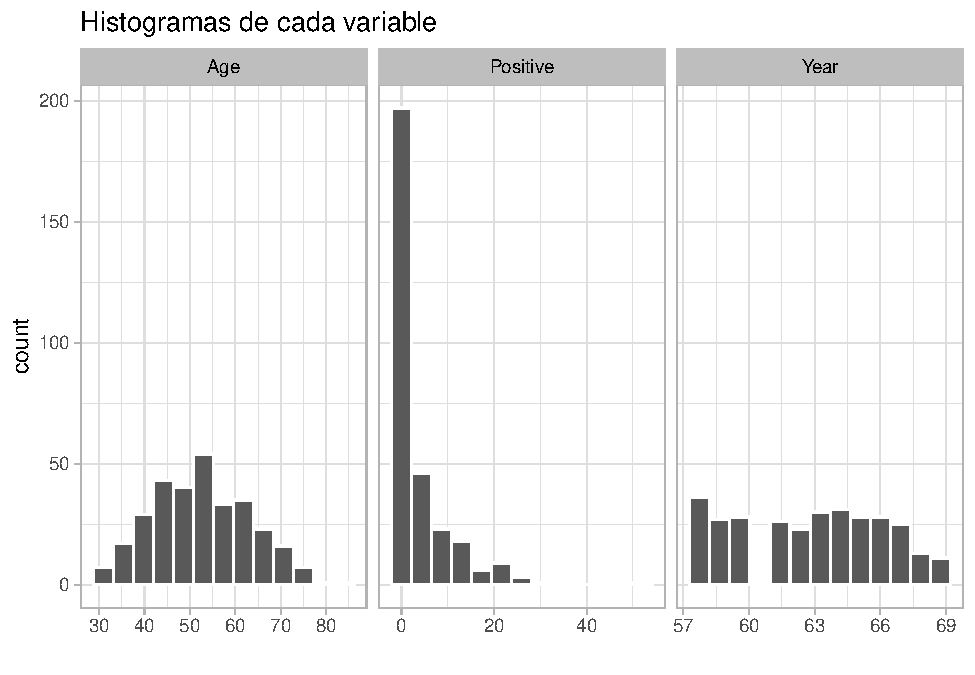
\includegraphics{EDA2_files/figure-latex/unnamed-chunk-9-1} \end{center}

Una a una

\begin{Shaded}
\begin{Highlighting}[]
\NormalTok{colors <-}\StringTok{ }\KeywordTok{c}\NormalTok{(}\StringTok{"chocolate"}\NormalTok{, }\StringTok{"deepskyblue1"}\NormalTok{, }\StringTok{"plum1"}\NormalTok{)}
\NormalTok{bins <-}\StringTok{ }\KeywordTok{c}\NormalTok{(}\DecValTok{15}\NormalTok{,}\DecValTok{10}\NormalTok{,}\DecValTok{20}\NormalTok{)}
\NormalTok{plt <-}\StringTok{ }\KeywordTok{list}\NormalTok{(}\DataTypeTok{length =} \KeywordTok{length}\NormalTok{(names))}

\ControlFlowTok{for}\NormalTok{ (i }\ControlFlowTok{in} \DecValTok{1}\OperatorTok{:}\KeywordTok{length}\NormalTok{(names)) \{}
  \KeywordTok{ggplot}\NormalTok{(haberman, }\KeywordTok{aes_string}\NormalTok{(}\DataTypeTok{x=}\NormalTok{names[i])) }\OperatorTok{+}\StringTok{ }
\StringTok{    }\KeywordTok{geom_histogram}\NormalTok{(}\KeywordTok{aes}\NormalTok{(}\DataTypeTok{y=}\NormalTok{..density..), }\DataTypeTok{size=}\DecValTok{1}\NormalTok{, }\DataTypeTok{bins=}\NormalTok{bins[i], }\DataTypeTok{color=}\StringTok{"black"}\NormalTok{, }\DataTypeTok{fill=}\NormalTok{colors[i]) }\OperatorTok{+}
\StringTok{    }\KeywordTok{geom_density}\NormalTok{(}\DataTypeTok{alpha=}\NormalTok{.}\DecValTok{3}\NormalTok{, }\DataTypeTok{fill=}\StringTok{"black"}\NormalTok{, }\DataTypeTok{color=}\StringTok{"green"}\NormalTok{, }\DataTypeTok{size=}\NormalTok{.}\DecValTok{5}\NormalTok{) }\OperatorTok{+}
\StringTok{    }\KeywordTok{labs}\NormalTok{(}\DataTypeTok{title=}\StringTok{""}\NormalTok{, }\DataTypeTok{x=}\StringTok{""}\NormalTok{, }\DataTypeTok{y=}\StringTok{""}\NormalTok{) }\OperatorTok{+}
\StringTok{    }\KeywordTok{theme_light}\NormalTok{() ->}\StringTok{ }\NormalTok{plt[[i]]}
  
  \KeywordTok{print}\NormalTok{(plt[[i]] }\OperatorTok{+}\StringTok{ }\KeywordTok{labs}\NormalTok{(}\DataTypeTok{title=}\KeywordTok{sprintf}\NormalTok{(}\StringTok{"Histograma %s"}\NormalTok{, names[i]), }\DataTypeTok{x=}\StringTok{""}\NormalTok{))}
\NormalTok{\}}
\end{Highlighting}
\end{Shaded}

\begin{center}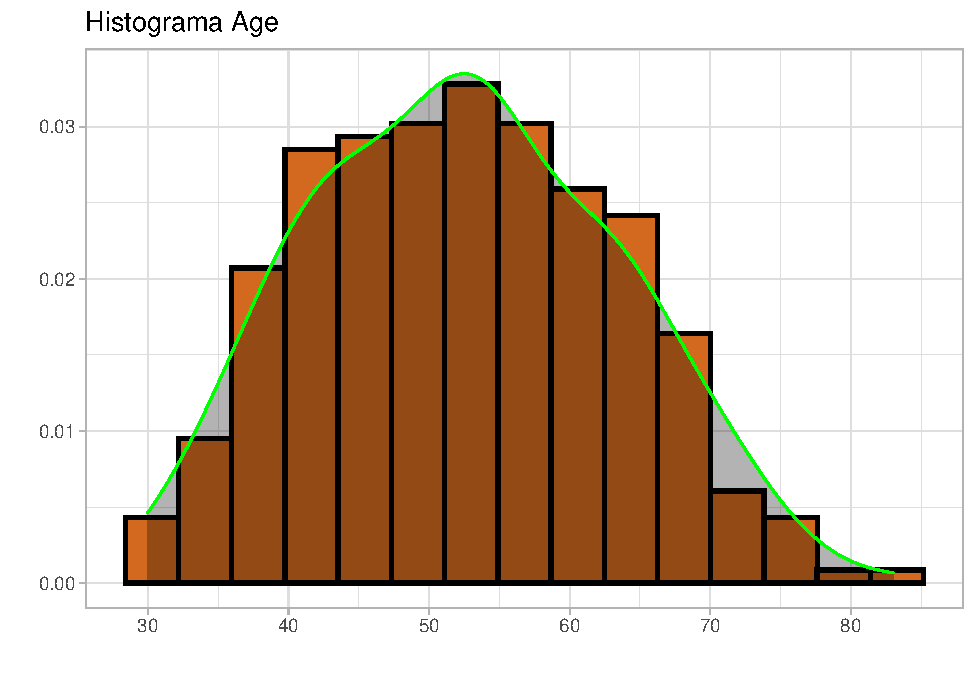
\includegraphics{EDA2_files/figure-latex/unnamed-chunk-10-1} \end{center}

\begin{center}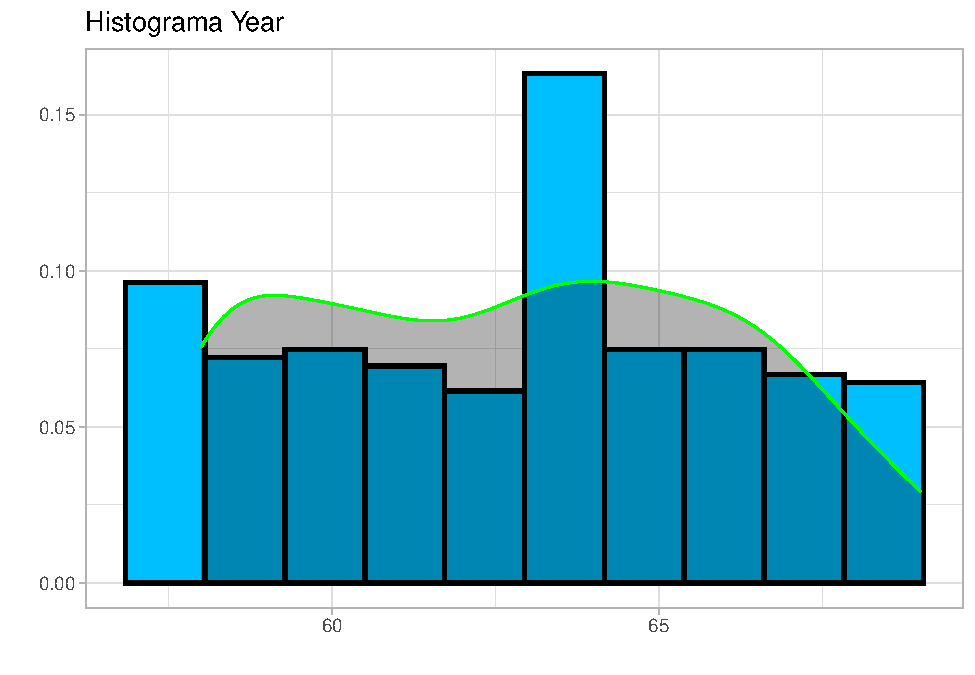
\includegraphics{EDA2_files/figure-latex/unnamed-chunk-10-2} \end{center}

\begin{center}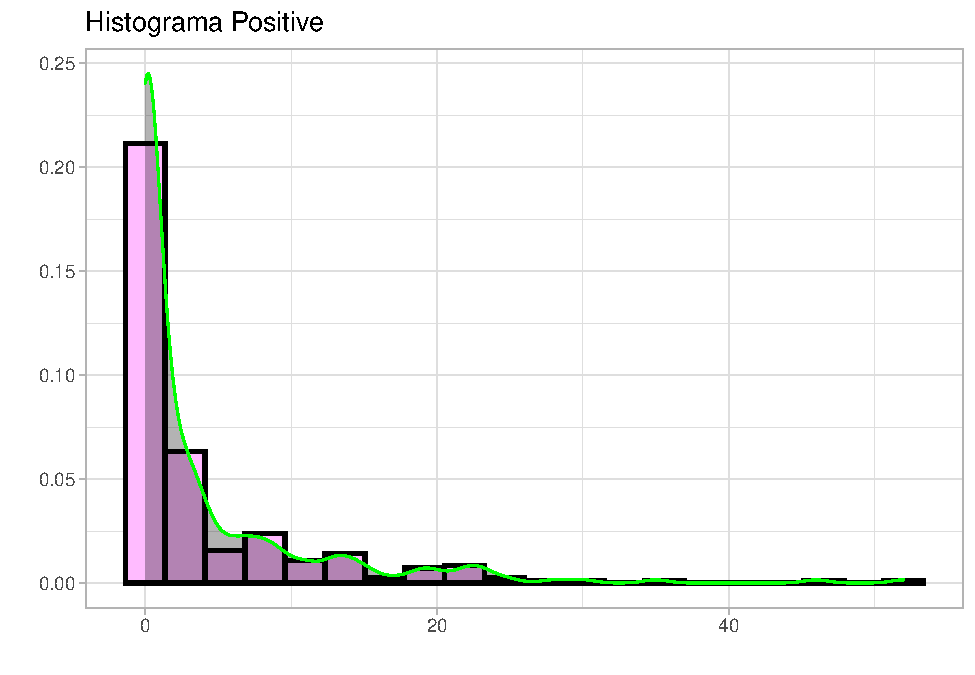
\includegraphics{EDA2_files/figure-latex/unnamed-chunk-10-3} \end{center}

\begin{Shaded}
\begin{Highlighting}[]
\KeywordTok{plot_grid}\NormalTok{(}\DataTypeTok{plotlist=}\NormalTok{plt, }\DataTypeTok{ncol=}\DecValTok{2}\NormalTok{, }\DataTypeTok{labels =}\NormalTok{ names, }\DataTypeTok{label_size =} \DecValTok{8}\NormalTok{)}
\end{Highlighting}
\end{Shaded}

\begin{center}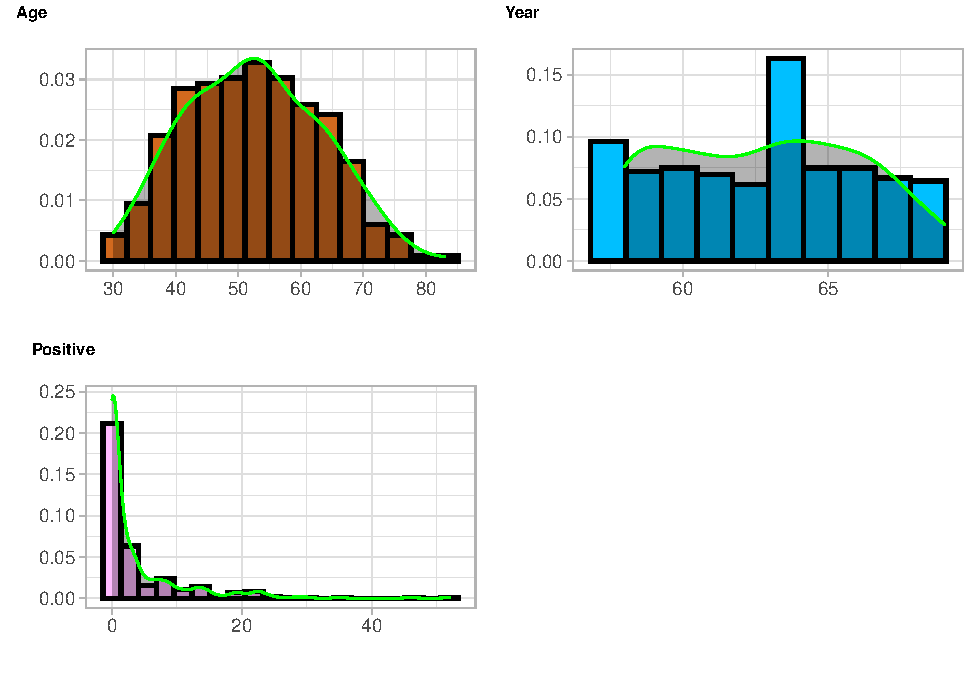
\includegraphics{EDA2_files/figure-latex/unnamed-chunk-10-4} \end{center}

\begin{Shaded}
\begin{Highlighting}[]
\NormalTok{colors <-}\StringTok{ }\KeywordTok{c}\NormalTok{(}\StringTok{"chocolate"}\NormalTok{, }\StringTok{"deepskyblue1"}\NormalTok{, }\StringTok{"plum1"}\NormalTok{)}
\NormalTok{plt <-}\StringTok{ }\KeywordTok{list}\NormalTok{(}\DataTypeTok{length =} \KeywordTok{length}\NormalTok{(names))}

\ControlFlowTok{for}\NormalTok{ (i }\ControlFlowTok{in} \DecValTok{1}\OperatorTok{:}\KeywordTok{length}\NormalTok{(names)) \{}
  \KeywordTok{ggplot}\NormalTok{(haberman, }\KeywordTok{aes_string}\NormalTok{(}\DataTypeTok{x=}\NormalTok{names[i])) }\OperatorTok{+}\StringTok{ }
\StringTok{    }\KeywordTok{geom_boxplot}\NormalTok{(}\DataTypeTok{fill =}\NormalTok{ colors[i]) }\OperatorTok{+}
\StringTok{    }\KeywordTok{labs}\NormalTok{(}\DataTypeTok{title=}\StringTok{""}\NormalTok{, }\DataTypeTok{x=}\StringTok{""}\NormalTok{, }\DataTypeTok{y=}\StringTok{""}\NormalTok{) }\OperatorTok{+}
\StringTok{    }\KeywordTok{theme_light}\NormalTok{() ->}\StringTok{ }\NormalTok{plt[[i]]}
  
  \KeywordTok{print}\NormalTok{(plt[[i]] }\OperatorTok{+}\StringTok{ }\KeywordTok{labs}\NormalTok{(}\DataTypeTok{title=}\KeywordTok{sprintf}\NormalTok{(}\StringTok{"Boxplot %s"}\NormalTok{, names[i]), }\DataTypeTok{x=}\StringTok{""}\NormalTok{))}
\NormalTok{\}}
\end{Highlighting}
\end{Shaded}

\begin{center}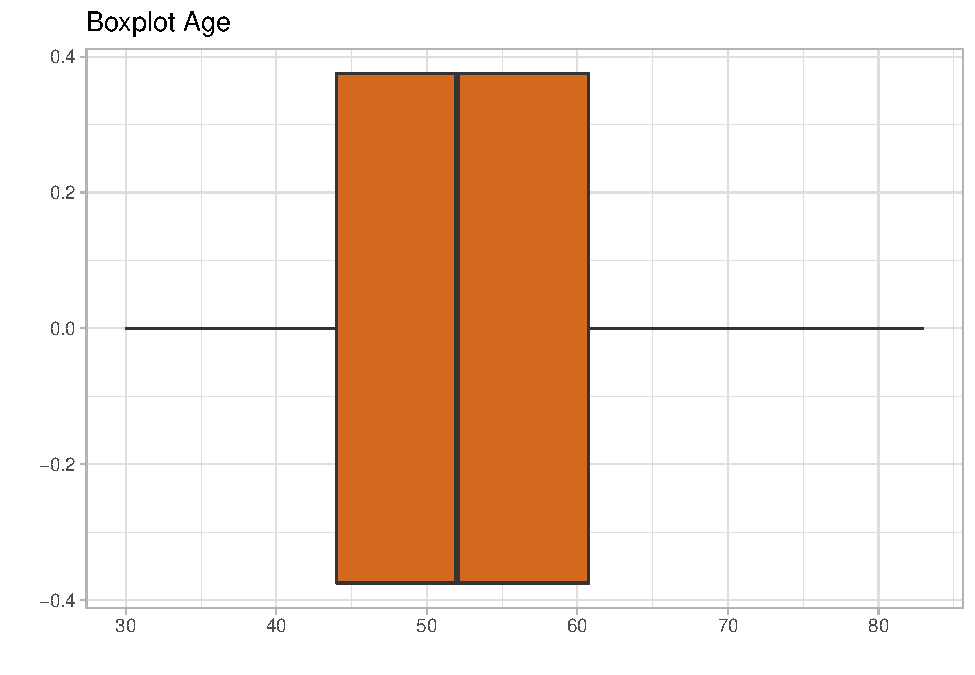
\includegraphics{EDA2_files/figure-latex/unnamed-chunk-11-1} \end{center}

\begin{center}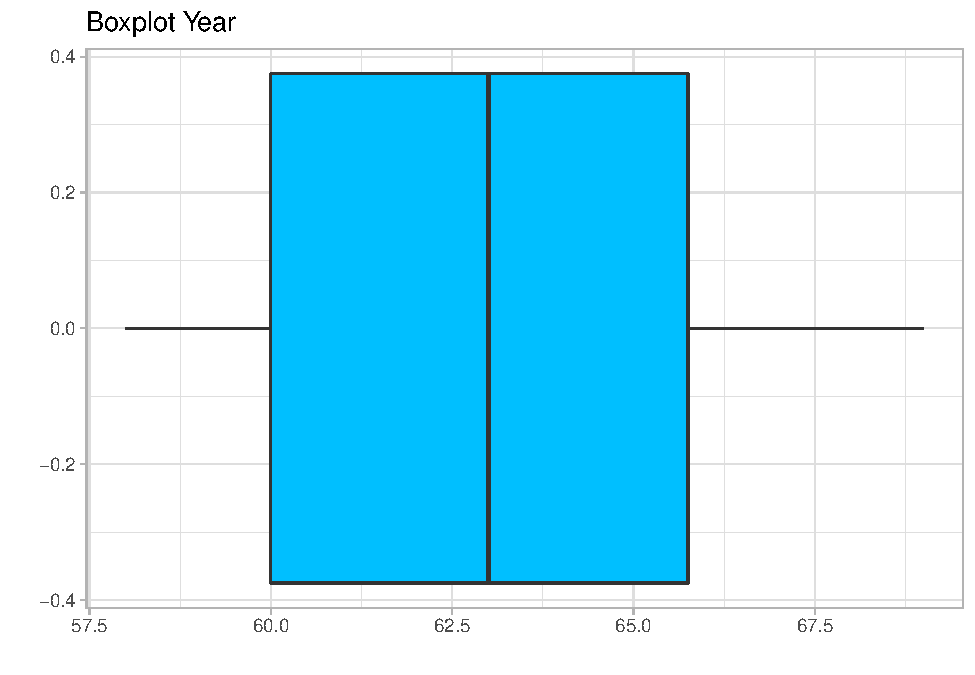
\includegraphics{EDA2_files/figure-latex/unnamed-chunk-11-2} \end{center}

\begin{center}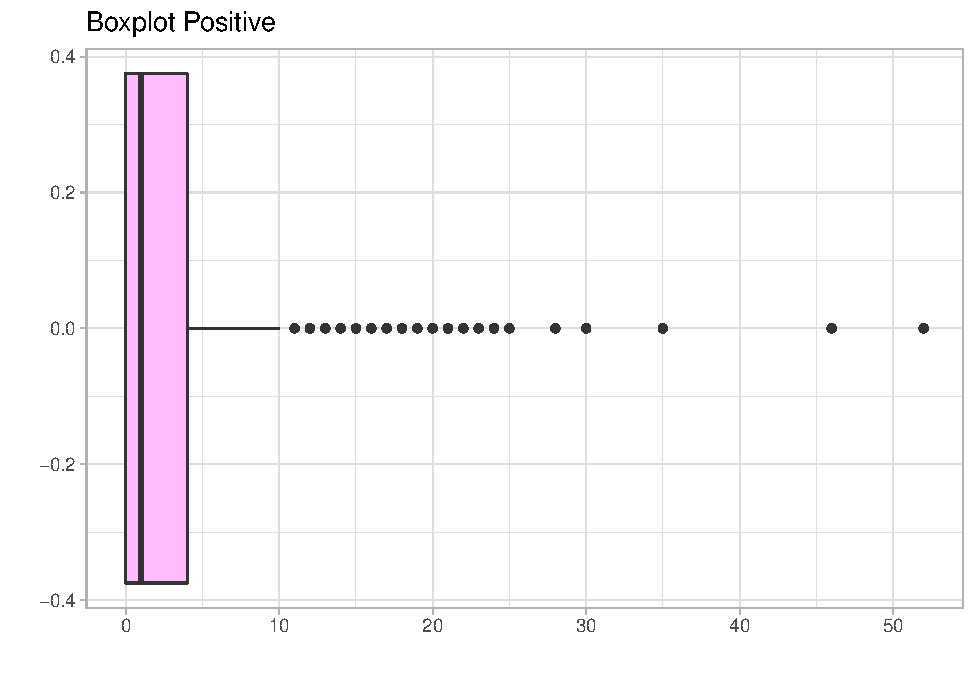
\includegraphics{EDA2_files/figure-latex/unnamed-chunk-11-3} \end{center}

\begin{Shaded}
\begin{Highlighting}[]
\KeywordTok{plot_grid}\NormalTok{(}\DataTypeTok{plotlist=}\NormalTok{plt, }\DataTypeTok{ncol=}\DecValTok{2}\NormalTok{, }\DataTypeTok{labels =}\NormalTok{ names, }\DataTypeTok{label_size =} \DecValTok{8}\NormalTok{)}
\end{Highlighting}
\end{Shaded}

\begin{center}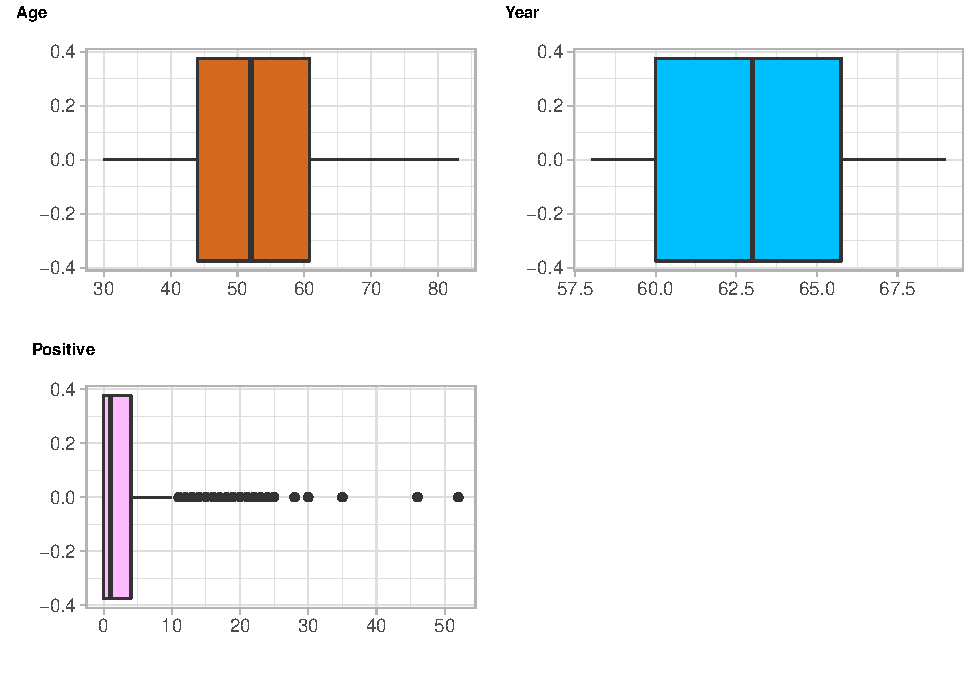
\includegraphics{EDA2_files/figure-latex/unnamed-chunk-11-4} \end{center}

\begin{Shaded}
\begin{Highlighting}[]
\KeywordTok{ggplot}\NormalTok{(}\KeywordTok{melt}\NormalTok{(haberman), }\KeywordTok{aes}\NormalTok{(}\DataTypeTok{x=}\NormalTok{variable, }\DataTypeTok{y=}\NormalTok{value)) }\OperatorTok{+}\StringTok{ }
\StringTok{  }\KeywordTok{geom_boxplot}\NormalTok{() }\OperatorTok{+}
\StringTok{  }\KeywordTok{labs}\NormalTok{(}\DataTypeTok{title=}\StringTok{"Boxplot con mismo rango"}\NormalTok{) }\OperatorTok{+}
\StringTok{  }\KeywordTok{theme}\NormalTok{(}\DataTypeTok{axis.text.x =} \KeywordTok{element_text}\NormalTok{(}\DataTypeTok{angle =} \DecValTok{90}\NormalTok{))}
\end{Highlighting}
\end{Shaded}

\begin{verbatim}
No id variables; using all as measure variables
\end{verbatim}

\begin{center}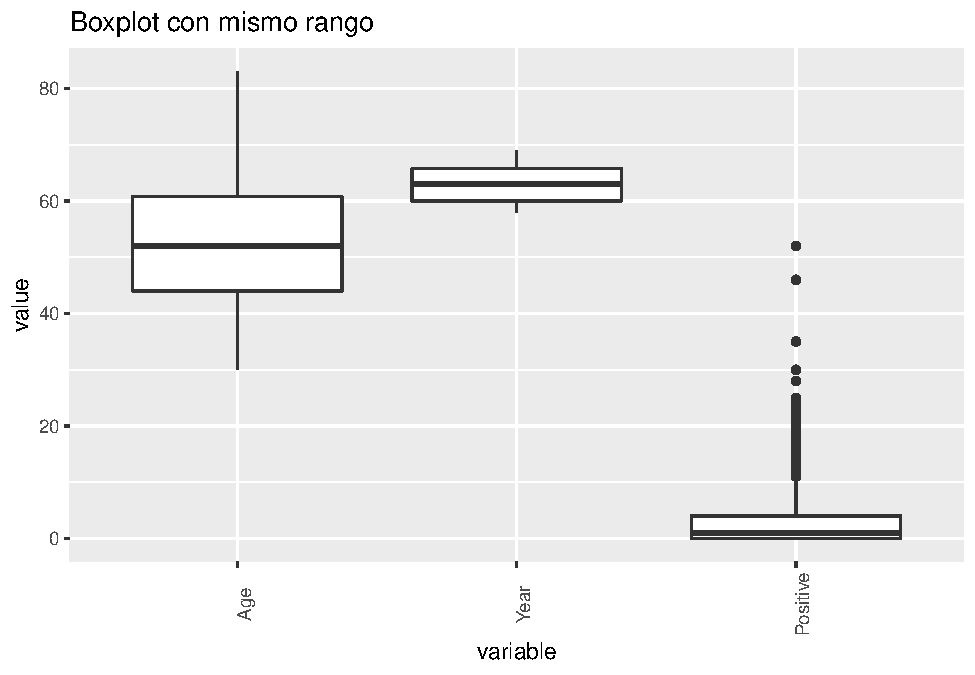
\includegraphics{EDA2_files/figure-latex/unnamed-chunk-12-1} \end{center}

Ya la descripción del problema nos lo decía, los rangos en los que se
distribuyen los datos son muy diferentes dependiendo de la variable. Es
necesario aplicar un proceso de estandarización para clasificación.

\begin{center}\rule{0.5\linewidth}{0.5pt}\end{center}

\hypertarget{missing-values}{%
\subsection{Missing values}\label{missing-values}}

Nos cuestionamos la ocurrencia de instancias con cero en el número de
positivos. Podríamos pensar que se trata de una codificación de missing
values si nos aseguramos que la operación consistan en eliminar estos
nodos positivos.

Si revisamos la información que tenemos, estos nodos positivos se
denominan auxiliares, y una mayor investigación del problema por
internet nos asegura de que estos valores de cero no se corresponden a
missing values.

Si hubiéramos descubierto que sí lo son, y tras ver que una gran parte
de las instancias contienen este valor, habríamos tenido que buscar
algún tipo de imputación para rellenar estos valores. Teniendo un número
pequeño de valores reales, probablemente habríamos optado por KNN o
interpolación lineal.

\begin{center}\rule{0.5\linewidth}{0.5pt}\end{center}

Podemos comparar los rangos intercuartiles si estandarizamos antes el
dataset

\begin{Shaded}
\begin{Highlighting}[]
\KeywordTok{scale}\NormalTok{(haberman) }\OperatorTok\StringTok{ }\KeywordTok{apply}\NormalTok{(}\DecValTok{2}\NormalTok{, IQR)}
\end{Highlighting}
\end{Shaded}

\begin{verbatim}
     Age     Year Positive 
1.550430 1.769555 0.556355 
\end{verbatim}

También podemos ver la distancia entre mínimos y máximos

\begin{Shaded}
\begin{Highlighting}[]
\KeywordTok{scale}\NormalTok{(haberman) }\OperatorTok\StringTok{ }\KeywordTok{apply}\NormalTok{(}\DecValTok{2}\NormalTok{, range) }\OperatorTok\StringTok{ }\KeywordTok{apply}\NormalTok{(}\DecValTok{2}\NormalTok{, dist)}
\end{Highlighting}
\end{Shaded}

\begin{verbatim}
     Age     Year Positive 
4.905839 3.385235 7.232616 
\end{verbatim}

\hypertarget{age}{%
\paragraph{Age}\label{age}}

Vemos que no contamos con valores de todos los años:

\begin{Shaded}
\begin{Highlighting}[]
\KeywordTok{table}\NormalTok{(haberman}\OperatorTok{$}\NormalTok{Age)}
\KeywordTok{table}\NormalTok{(haberman}\OperatorTok{$}\NormalTok{Age) }\OperatorTok\StringTok{ }\NormalTok{length}

\NormalTok{(}\DecValTok{83-30}\OperatorTok{+}\DecValTok{1}\NormalTok{) }\OperatorTok{==}\StringTok{ }\KeywordTok{table}\NormalTok{(haberman}\OperatorTok{$}\NormalTok{Age) }\OperatorTok\StringTok{ }\NormalTok{length}
\end{Highlighting}
\end{Shaded}

\begin{verbatim}

30 31 33 34 35 36 37 38 39 40 41 42 43 44 45 46 47 48 49 50 51 52 53 54 55 56 
 3  2  2  7  2  2  6 10  6  3 10  9 11  7  9  7 11  7 10 12  6 14 11 13 10  7 
57 58 59 60 61 62 63 64 65 66 67 68 69 70 71 72 73 74 75 76 77 78 83 
11  7  8  6  9  7  8  5 10  5  6  2  4  7  1  4  2  2  1  1  1  1  1 
[1] 49
[1] FALSE
\end{verbatim}

\hypertarget{year}{%
\paragraph{Year}\label{year}}

Aunque no se vea bien en las gráficas, contamos con valores de todos los
años, con mayor cantidad en los iniciales:

\begin{Shaded}
\begin{Highlighting}[]
\KeywordTok{table}\NormalTok{(haberman}\OperatorTok{$}\NormalTok{Year)}
\end{Highlighting}
\end{Shaded}

\begin{verbatim}

58 59 60 61 62 63 64 65 66 67 68 69 
36 27 28 26 23 30 31 28 28 25 13 11 
\end{verbatim}

\hypertarget{positive}{%
\subparagraph{Positive}\label{positive}}

La variable Positive parece llevar una distribución exponencial, y
problablemente por ello aparezcan tantos posibles outliers.

\begin{center}\rule{0.5\linewidth}{0.5pt}\end{center}

\hypertarget{anuxe1lisis-sobre-las-distribuciones}{%
\subsubsection{Análisis sobre las
distribuciones}\label{anuxe1lisis-sobre-las-distribuciones}}

Ninguna variable parece seguir una distribución semejante a una
distribución normal, lo comprobamos con un test estadístico
(Shapiro-Wilk test):

\begin{Shaded}
\begin{Highlighting}[]
\KeywordTok{normality}\NormalTok{(haberman) }\OperatorTok\StringTok{ }\KeywordTok{filter}\NormalTok{(p_value }\OperatorTok{<}\StringTok{ }\FloatTok{0.05}\NormalTok{)}
\end{Highlighting}
\end{Shaded}

\begin{verbatim}
Warning: `cols` is now required when using unnest().
Please use `cols = c(statistic)`
\end{verbatim}

\begin{tabular}{l|r|r|r}
\hline
vars & statistic & p\_value & sample\\
\hline
Age & 0.9894580 & 0.0260466 & 306\\
\hline
Year & 0.9467912 & 0.0000000 & 306\\
\hline
Positive & 0.6153079 & 0.0000000 & 306\\
\hline
\end{tabular}

El test de Shapiro nos dice claramente que ninguna variable sigue una
distribución normal.

Lo mostramos gráficamente con plots Q-Q:

\begin{Shaded}
\begin{Highlighting}[]
\NormalTok{plt <-}\StringTok{ }\KeywordTok{list}\NormalTok{(}\DataTypeTok{length =} \KeywordTok{length}\NormalTok{(names))}

\NormalTok{x<-}\KeywordTok{rnorm}\NormalTok{(}\DecValTok{100}\NormalTok{, }\DataTypeTok{mean=}\DecValTok{0}\NormalTok{, }\DataTypeTok{sd=}\DecValTok{1}\NormalTok{)}

\ControlFlowTok{for}\NormalTok{ (i }\ControlFlowTok{in} \DecValTok{1}\OperatorTok{:}\KeywordTok{length}\NormalTok{(names)) \{}
  \KeywordTok{ggplot}\NormalTok{(haberman, }\KeywordTok{aes_string}\NormalTok{(}\DataTypeTok{sample=}\NormalTok{names[i])) }\OperatorTok{+}\StringTok{ }
\StringTok{    }\KeywordTok{stat_qq}\NormalTok{(}\DataTypeTok{alpha=}\NormalTok{.}\DecValTok{3}\NormalTok{, }\DataTypeTok{fill=}\NormalTok{colors[i], }\DataTypeTok{size=}\DecValTok{1}\NormalTok{) }\OperatorTok{+}
\StringTok{    }\KeywordTok{stat_qq_line}\NormalTok{() }\OperatorTok{+}
\StringTok{    }\KeywordTok{labs}\NormalTok{(}\DataTypeTok{title=}\StringTok{""}\NormalTok{, }\DataTypeTok{x=}\StringTok{""}\NormalTok{, }\DataTypeTok{y=}\StringTok{""}\NormalTok{) }\OperatorTok{+}
\StringTok{    }\KeywordTok{theme_light}\NormalTok{() ->}\StringTok{ }\NormalTok{plt[[i]]}
  
  \KeywordTok{print}\NormalTok{(plt[[i]] }\OperatorTok{+}\StringTok{ }\KeywordTok{labs}\NormalTok{(}\DataTypeTok{title=}\KeywordTok{sprintf}\NormalTok{(}\StringTok{"QQ-plot %s"}\NormalTok{, names[i]), }\DataTypeTok{x=}\StringTok{""}\NormalTok{))}
\NormalTok{\}}
\end{Highlighting}
\end{Shaded}

\begin{center}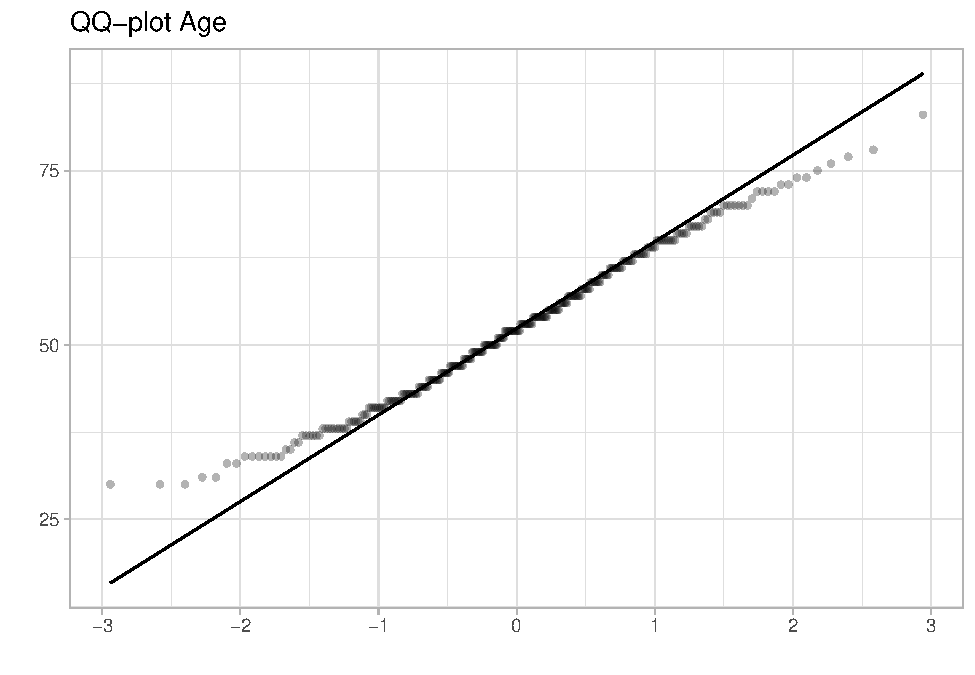
\includegraphics{EDA2_files/figure-latex/unnamed-chunk-18-1} \end{center}

\begin{center}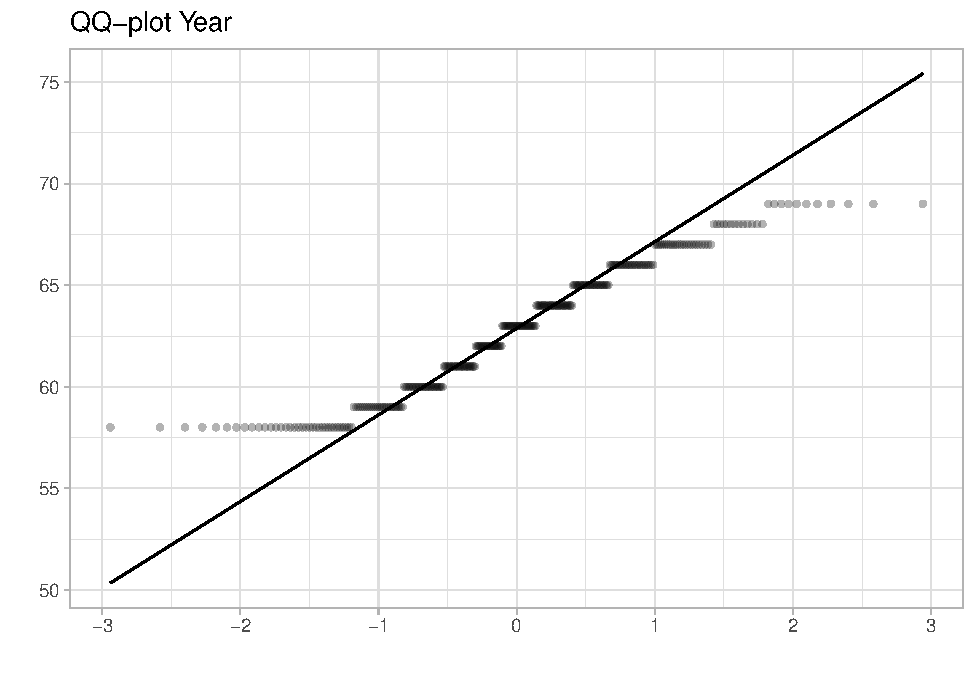
\includegraphics{EDA2_files/figure-latex/unnamed-chunk-18-2} \end{center}

\begin{center}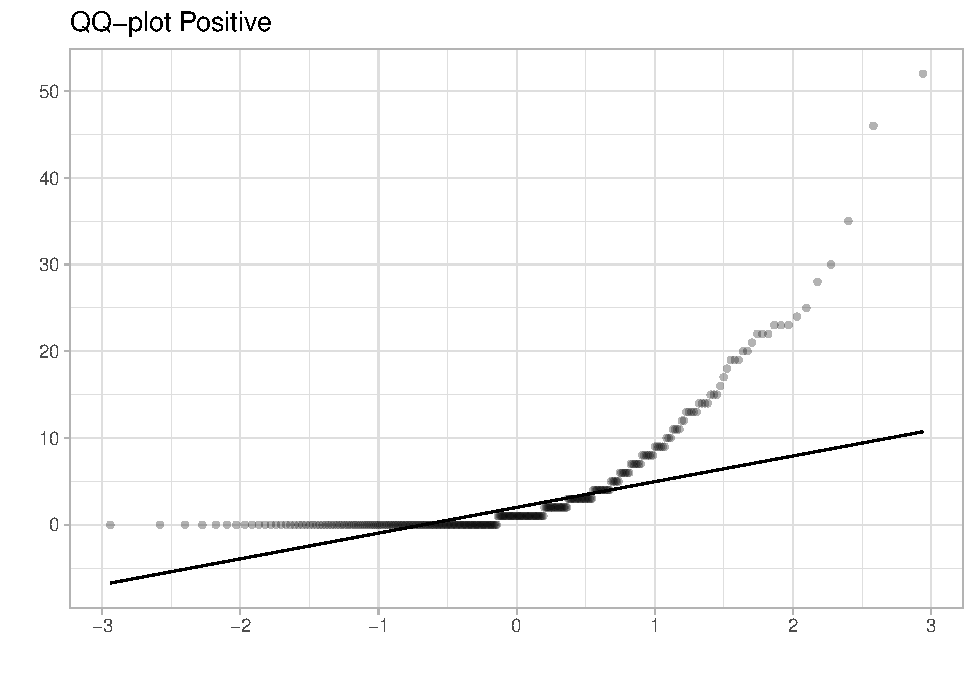
\includegraphics{EDA2_files/figure-latex/unnamed-chunk-18-3} \end{center}

\begin{Shaded}
\begin{Highlighting}[]
\KeywordTok{plot_grid}\NormalTok{(}\DataTypeTok{plotlist=}\NormalTok{plt, }\DataTypeTok{ncol=}\DecValTok{2}\NormalTok{, }\DataTypeTok{labels =}\NormalTok{ names, }\DataTypeTok{label_size =} \DecValTok{8}\NormalTok{)}
\end{Highlighting}
\end{Shaded}

\begin{center}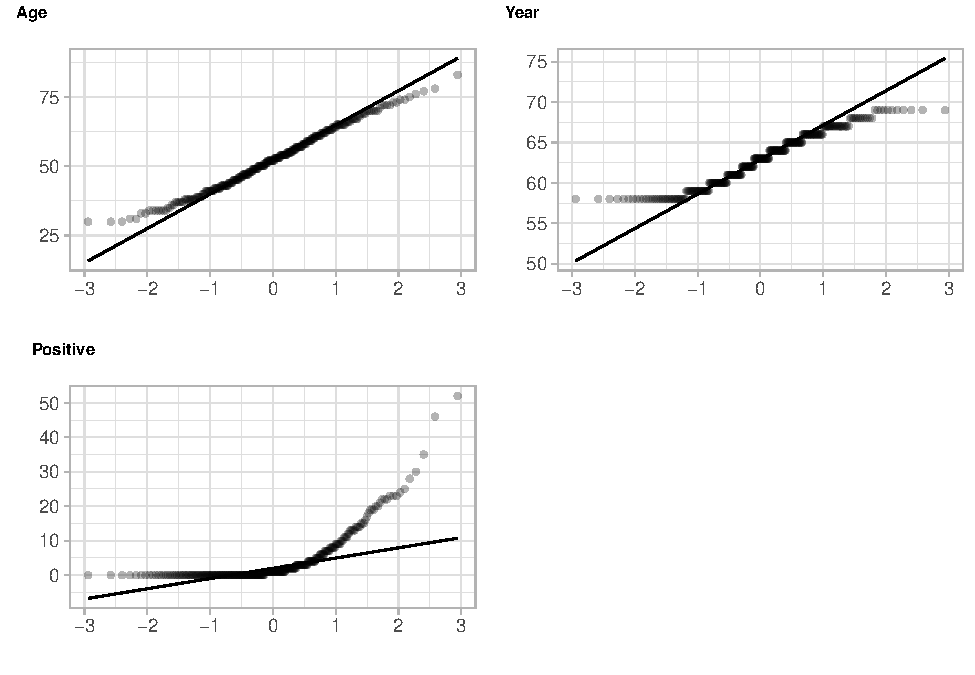
\includegraphics{EDA2_files/figure-latex/unnamed-chunk-18-4} \end{center}

Se ve que las distribuciones no siguen los cuartiles normales,
mayormente en las colas.

La variable Positive parece seguir una distribución exponencial, hacemos
un test de Kolmogorov-Smirnov para corroborarlo:

\begin{Shaded}
\begin{Highlighting}[]
\CommentTok{# data generation}
\NormalTok{ex <-}\StringTok{ }\KeywordTok{rexp}\NormalTok{(}\DecValTok{10000}\NormalTok{, }\DataTypeTok{rate =} \FloatTok{1.85}\NormalTok{) }\CommentTok{# generate some exponential distribution}
\NormalTok{control <-}\StringTok{ }\KeywordTok{abs}\NormalTok{(}\KeywordTok{rnorm}\NormalTok{(}\DecValTok{10000}\NormalTok{)) }\CommentTok{# generate some other distribution}

\CommentTok{# estimate the parameters}
\NormalTok{fit1 <-}\StringTok{ }\KeywordTok{fitdistr}\NormalTok{(ex, }\StringTok{"exponential"}\NormalTok{) }
\NormalTok{fit2 <-}\StringTok{ }\KeywordTok{fitdistr}\NormalTok{(haberman}\OperatorTok{$}\NormalTok{Positive }\OperatorTok\StringTok{ }\KeywordTok{unique}\NormalTok{(), }\StringTok{"exponential"}\NormalTok{)}

\CommentTok{# goodness of fit test}
\KeywordTok{ks.test}\NormalTok{(ex, }\StringTok{"pexp"}\NormalTok{, fit1}\OperatorTok{$}\NormalTok{estimate) }\CommentTok{# p-value > 0.05 -> distribution not refused}
\KeywordTok{ks.test}\NormalTok{(haberman}\OperatorTok{$}\NormalTok{Positive, }\StringTok{"pexp"}\NormalTok{, fit2}\OperatorTok{$}\NormalTok{estimate) }\CommentTok{#  significant p-value -> distribution refused}
\end{Highlighting}
\end{Shaded}

\begin{verbatim}
Warning in ks.test(haberman$Positive, "pexp", fit2$estimate): ties should not be
present for the Kolmogorov-Smirnov test
\end{verbatim}

\begin{Shaded}
\begin{Highlighting}[]
\CommentTok{# plot a graph}
\KeywordTok{hist}\NormalTok{(haberman}\OperatorTok{$}\NormalTok{Positive, }\DataTypeTok{freq =} \OtherTok{FALSE}\NormalTok{, }\DataTypeTok{breaks =} \DecValTok{100}\NormalTok{, }\DataTypeTok{xlim =} \KeywordTok{c}\NormalTok{(}\DecValTok{0}\NormalTok{, }\KeywordTok{quantile}\NormalTok{(haberman}\OperatorTok{$}\NormalTok{Positive, }\FloatTok{0.99}\NormalTok{)))}
\KeywordTok{curve}\NormalTok{(}\KeywordTok{dexp}\NormalTok{(x, }\DataTypeTok{rate =}\NormalTok{ fit1}\OperatorTok{$}\NormalTok{estimate), }\DataTypeTok{from =} \DecValTok{0}\NormalTok{, }\DataTypeTok{col =} \StringTok{"red"}\NormalTok{, }\DataTypeTok{add =} \OtherTok{TRUE}\NormalTok{)}
\end{Highlighting}
\end{Shaded}

\begin{center}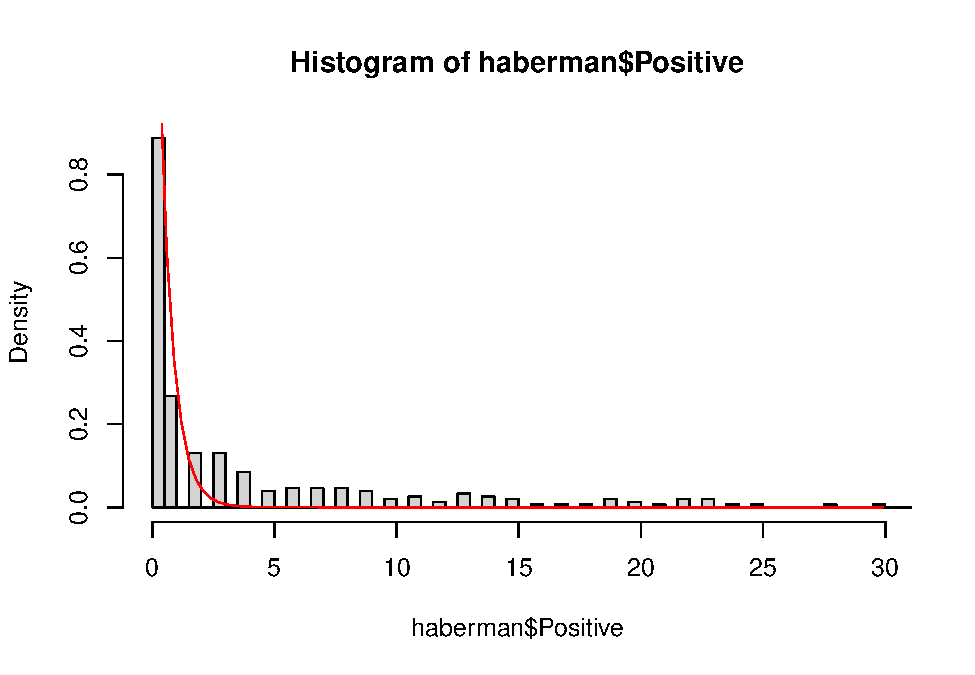
\includegraphics{EDA2_files/figure-latex/unnamed-chunk-19-1} \end{center}

\begin{Shaded}
\begin{Highlighting}[]
\CommentTok{# control}
\end{Highlighting}
\end{Shaded}

\begin{verbatim}

    One-sample Kolmogorov-Smirnov test

data:  ex
D = 0.0053904, p-value = 0.9334
alternative hypothesis: two-sided


    One-sample Kolmogorov-Smirnov test

data:  haberman$Positive
D = 0.54423, p-value < 2.2e-16
alternative hypothesis: two-sided
\end{verbatim}

Al ser el p-valor \textless0.05 el test nos lo rechaza. El plot también
nos lo muestra más claramente, la forma de la cola de la distribución
probablemente sea la causante de que no siga ese tipo de distribución

Podemos hacer un gráfico QQ con los cuartiles de una distribución
exponencial

\begin{Shaded}
\begin{Highlighting}[]
\CommentTok{# From https://stats.stackexchange.com/questions/76994/how-do-i-check-if-my-data-fits-an-exponential-distribution/76998}
\NormalTok{qqexp <-}\StringTok{  }\ControlFlowTok{function}\NormalTok{(y, }\DataTypeTok{line=}\OtherTok{FALSE}\NormalTok{, ...) \{ }
\NormalTok{    y <-}\StringTok{ }\NormalTok{y[}\OperatorTok{!}\KeywordTok{is.na}\NormalTok{(y)]}
\NormalTok{    n <-}\StringTok{ }\KeywordTok{length}\NormalTok{(y)}
\NormalTok{    x <-}\StringTok{ }\KeywordTok{qexp}\NormalTok{(}\KeywordTok{c}\NormalTok{(}\DecValTok{1}\OperatorTok{:}\NormalTok{n)}\OperatorTok{/}\NormalTok{(n}\OperatorTok{+}\DecValTok{1}\NormalTok{))}
\NormalTok{    m <-}\StringTok{ }\KeywordTok{mean}\NormalTok{(y)}
    \ControlFlowTok{if}\NormalTok{ (}\KeywordTok{any}\NormalTok{(}\KeywordTok{range}\NormalTok{(y)}\OperatorTok{<}\DecValTok{0}\NormalTok{)) }\KeywordTok{stop}\NormalTok{(}\StringTok{"Data contains negative values"}\NormalTok{)}
\NormalTok{    ylim <-}\StringTok{ }\KeywordTok{c}\NormalTok{(}\DecValTok{0}\NormalTok{,}\KeywordTok{max}\NormalTok{(y))}
    \KeywordTok{qqplot}\NormalTok{(x, y, }\DataTypeTok{xlab=}\StringTok{"Exponential plotting position"}\NormalTok{,}\DataTypeTok{ylim=}\NormalTok{ylim,}\DataTypeTok{ylab=}\StringTok{"Ordered sample"}\NormalTok{, ...)}
    \ControlFlowTok{if}\NormalTok{ (line) }\KeywordTok{abline}\NormalTok{(}\DecValTok{0}\NormalTok{,m,}\DataTypeTok{lty=}\DecValTok{2}\NormalTok{)}
    \KeywordTok{invisible}\NormalTok{()}
\NormalTok{\}}

\KeywordTok{qqexp}\NormalTok{(haberman}\OperatorTok{$}\NormalTok{Positive, }\DataTypeTok{line=}\OtherTok{TRUE}\NormalTok{)}
\end{Highlighting}
\end{Shaded}

\begin{center}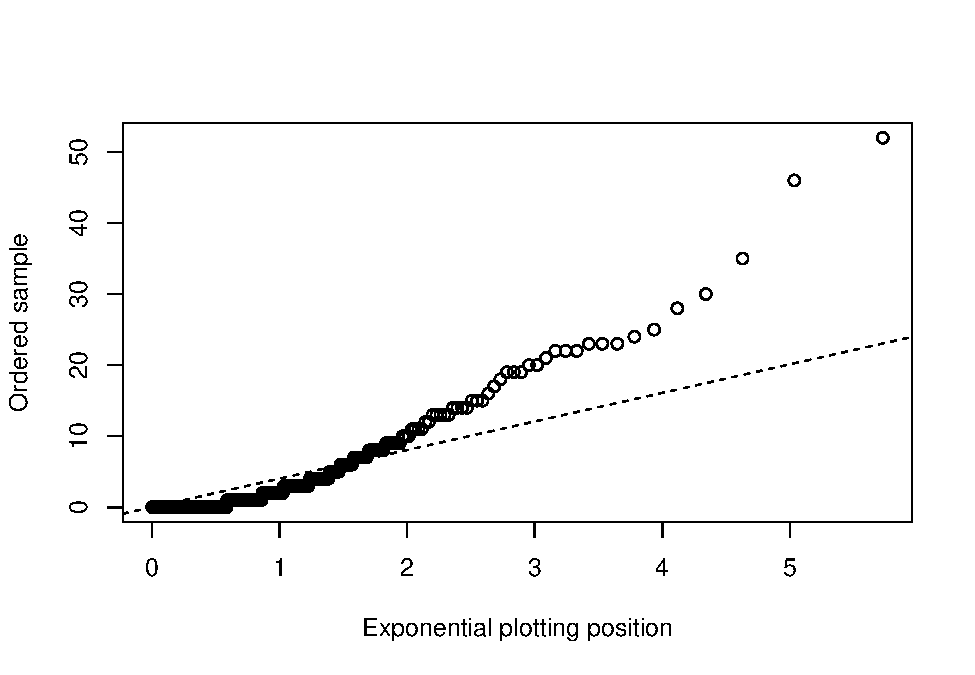
\includegraphics{EDA2_files/figure-latex/unnamed-chunk-20-1} \end{center}

Solo vemos skewness en la variable Positive, lo comprobamos:

\begin{Shaded}
\begin{Highlighting}[]
\NormalTok{skewCols <-}\StringTok{ }\KeywordTok{find_skewness}\NormalTok{(haberman)}
\KeywordTok{colnames}\NormalTok{(haberman)[skewCols]}
\end{Highlighting}
\end{Shaded}

\begin{verbatim}
[1] "Positive"
\end{verbatim}

Calculamos el grado que tienen:

\begin{Shaded}
\begin{Highlighting}[]
\KeywordTok{cat}\NormalTok{(}\StringTok{"Positive: "}\NormalTok{)}
\KeywordTok{skewness}\NormalTok{(haberman}\OperatorTok{$}\NormalTok{Positive)}
\KeywordTok{cat}\NormalTok{(}\StringTok{"Year: "}\NormalTok{)}
\KeywordTok{skewness}\NormalTok{(haberman}\OperatorTok{$}\NormalTok{Year)}
\KeywordTok{cat}\NormalTok{(}\StringTok{"Age: "}\NormalTok{)}
\KeywordTok{skewness}\NormalTok{(haberman}\OperatorTok{$}\NormalTok{Age)}
\end{Highlighting}
\end{Shaded}

\begin{verbatim}
Positive: [1] 2.969176
Year: [1] 0.07836828
Age: [1] 0.1457859
\end{verbatim}

Positive tiene skewness positiva en un alto grado, las demás tienen tan
poco como para poder considerarlo.

\begin{center}\rule{0.5\linewidth}{0.5pt}\end{center}

\hypertarget{transformaciones}{%
\subsubsection{Transformaciones}\label{transformaciones}}

Dejamos que el paquete caret nos proponga metodos de preprocesado

\begin{Shaded}
\begin{Highlighting}[]
\KeywordTok{preProcess}\NormalTok{(haberman)}
\end{Highlighting}
\end{Shaded}

\begin{verbatim}
Created from 306 samples and 3 variables

Pre-processing:
  - centered (3)
  - ignored (0)
  - scaled (3)
\end{verbatim}

Nos sugiere una estandarización a media cero y desviación típica 1. Para
un problema de clasificación esto es totalmente necesario puesto que no
queremos que los diferentes rangos de las variables hagan que haya
información de más peso que otra.

Según el método utilizado la necesitad de normalidad puede ser o no
necesaria. (CORROBORAR) Aplicar métodos de reducción de skewness en
Positive no parece interesante puesto que está demasiado ladeado.

\begin{Shaded}
\begin{Highlighting}[]
\NormalTok{haberman_transform <-}\StringTok{ }\KeywordTok{preProcess}\NormalTok{(haberman, }\DataTypeTok{method=}\KeywordTok{c}\NormalTok{(}\StringTok{"scale"}\NormalTok{, }\StringTok{"center"}\NormalTok{))}
\CommentTok{# haberman_transform <- preProcess(haberman, method=c("YeoJohnson","scale", "center"))}
\NormalTok{haberman_norm <-}\StringTok{ }\KeywordTok{predict}\NormalTok{(haberman_transform, haberman)}
\end{Highlighting}
\end{Shaded}

\begin{Shaded}
\begin{Highlighting}[]
\CommentTok{# colors <- c("chocolate", "deepskyblue1", "plum1")}
\CommentTok{# bins <- c(15,10,20)}
\CommentTok{# plt <- list(length = length(names))}
\CommentTok{# }
\CommentTok{# for (i in 1:length(names)) \{}
\CommentTok{#   ggplot(haberman_norm, aes_string(x=names[i])) + }
\CommentTok{#     geom_histogram(aes(y=..density..), size=1, bins=bins[i], color="black", fill=colors[i]) +}
\CommentTok{#     geom_density(alpha=.3, fill="black", color="green", size=.5) +}
\CommentTok{#     labs(title="", x="", y="") +}
\CommentTok{#     theme_light() -> plt[[i]]}
\CommentTok{#   }
\CommentTok{#   print(plt[[i]] + labs(title=sprintf("Histograma %s", names[i]), x=""))}
\CommentTok{# \}}
\CommentTok{# }
\CommentTok{# plot_grid(plotlist=plt, ncol=2, labels = names, label_size = 8)}
\end{Highlighting}
\end{Shaded}

\begin{center}\rule{0.5\linewidth}{0.5pt}\end{center}

\hypertarget{outliers}{%
\subsubsection{Outliers}\label{outliers}}

La única variable en la que podríamos considerar outliers es Positive.
Tanto para la edad como para los años no tiene sentido, además de que
hemos visto en los boxplots que en ellas todos los valores caen en el
95\% de la distribución.

A la hora de considerar los outliers en Positive, tal y como habíamos
mencionado en la descripción del problema, un alto número de nodos
detectados complica la operación y el pronóstico para el paciente.

Podemos mostrar para aquellos valores outliers la cantidad de
sobrevivientes:

\begin{Shaded}
\begin{Highlighting}[]
\NormalTok{haberman }\OperatorTok\StringTok{ }
\StringTok{  }\KeywordTok{bind_cols}\NormalTok{(labels) }\OperatorTok\StringTok{ }
\StringTok{  }\KeywordTok{filter}\NormalTok{(Positive}\OperatorTok{>}\DecValTok{10}\NormalTok{) }\OperatorTok
\StringTok{  }\KeywordTok{summarise}\NormalTok{(Survival) }\OperatorTok\StringTok{ }
\StringTok{  }\KeywordTok{table}\NormalTok{()}
\end{Highlighting}
\end{Shaded}

\begin{verbatim}
.
 No Yes 
 17  23 
\end{verbatim}

Vemos que realmente está equilibrado. Aún así, si hubiera una tendencia
negativa por un alto número en Positive querríamos que nuestro
clasificador fuera capaz de aprenderlo, por lo que proseguimos sin
eliminar outliers.

\begin{center}\rule{0.5\linewidth}{0.5pt}\end{center}

\hypertarget{anuxe1lisis-de-correlaciuxf3n}{%
\subsubsection{Análisis de
correlación}\label{anuxe1lisis-de-correlaciuxf3n}}

Como este es un problema de clasificación, necesitamos eliminar aquellas
variables correladas para que la información se aporte de manera
equitativa. Las gráficas no nos han dado ninguna señal de una posible
correlación, pero debemos asegurarnos de forma estadística.

Tenemos que tener en cuenta que las variables no siguen distribuciones
normales. Aunque el coeficiente de Pearson no asume normalidad (si asume
varianza y covarianza finitas), podemos usar el coeficiente de Kendall
para los cálculos. Independientemente del método usado vamos a obtener
las mismas correlaciones en este dataset, solo varía la fuerza con la
que se dan.

Corrplot

\begin{Shaded}
\begin{Highlighting}[]
\KeywordTok{corrplot.mixed}\NormalTok{(}\KeywordTok{cor}\NormalTok{(haberman), }\DataTypeTok{tl.pos=}\StringTok{"lt"}\NormalTok{, }\DataTypeTok{upper=}\StringTok{"color"}\NormalTok{, }\DataTypeTok{lower.col=}\StringTok{"black"}\NormalTok{, }\DataTypeTok{title=}\StringTok{"Pearson"}\NormalTok{)}
\end{Highlighting}
\end{Shaded}

\begin{center}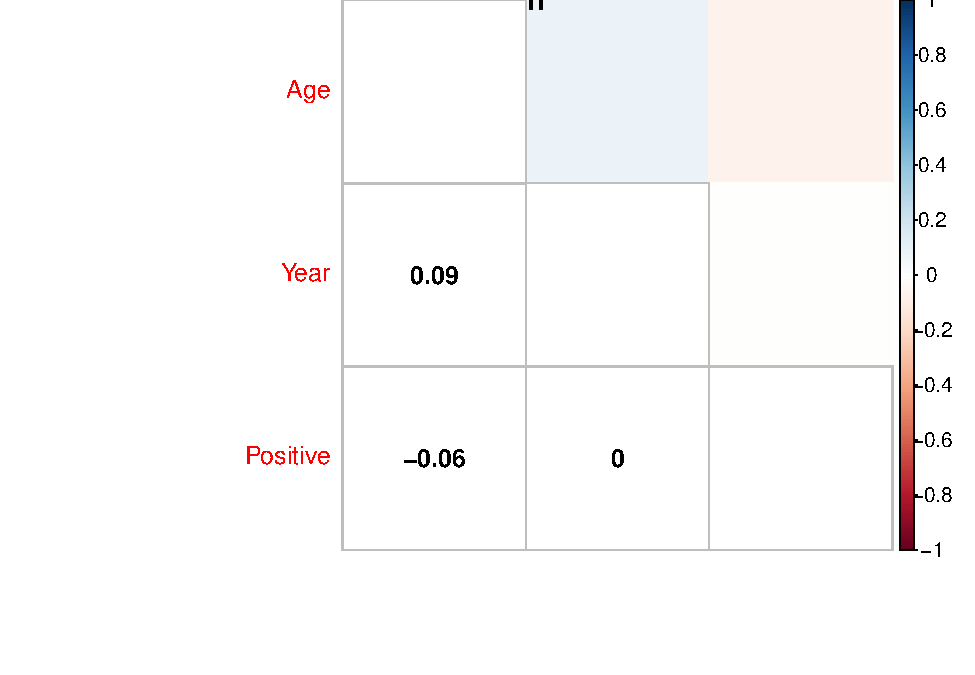
\includegraphics{EDA2_files/figure-latex/unnamed-chunk-27-1} \end{center}

\begin{Shaded}
\begin{Highlighting}[]
\KeywordTok{corrplot.mixed}\NormalTok{(}\KeywordTok{cor}\NormalTok{(haberman, }\DataTypeTok{method=}\StringTok{"kendall"}\NormalTok{), }\DataTypeTok{tl.pos=}\StringTok{"lt"}\NormalTok{, }\DataTypeTok{upper=}\StringTok{"color"}\NormalTok{, }\DataTypeTok{lower.col=}\StringTok{"black"}\NormalTok{, }\DataTypeTok{title=}\StringTok{"Kendall"}\NormalTok{)}
\end{Highlighting}
\end{Shaded}

\begin{center}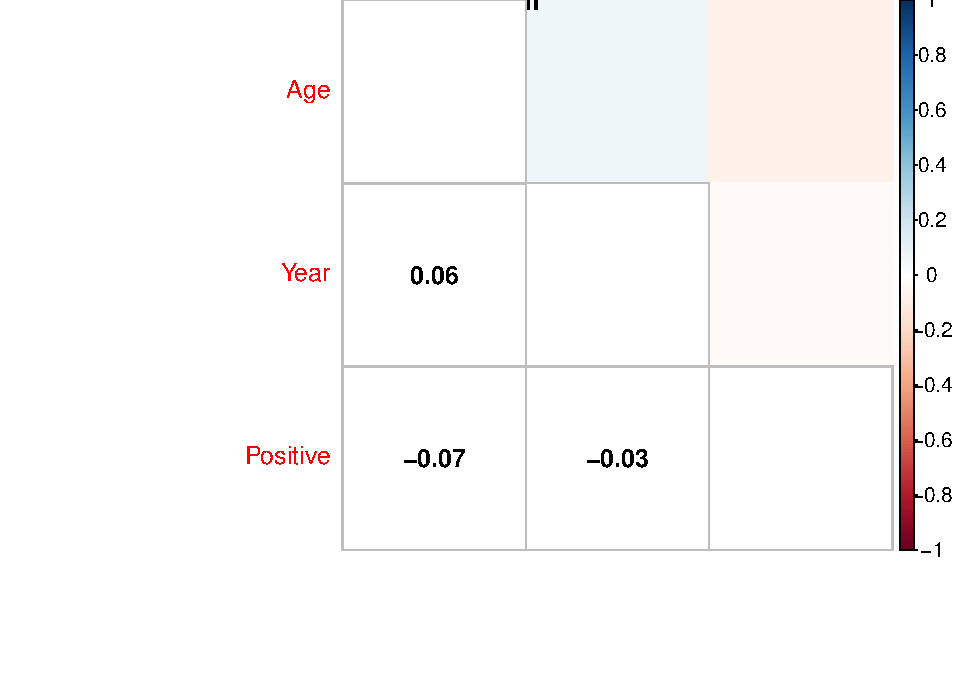
\includegraphics{EDA2_files/figure-latex/unnamed-chunk-27-2} \end{center}

Nos muestra que no existe correlación alguna entre las variables.

\begin{Shaded}
\begin{Highlighting}[]
\KeywordTok{scatterplotMatrix}\NormalTok{(haberman, }\DataTypeTok{pch=}\DecValTok{20}\NormalTok{, }\DataTypeTok{col=}\StringTok{"deepskyblue"}\NormalTok{)}
\end{Highlighting}
\end{Shaded}

\begin{center}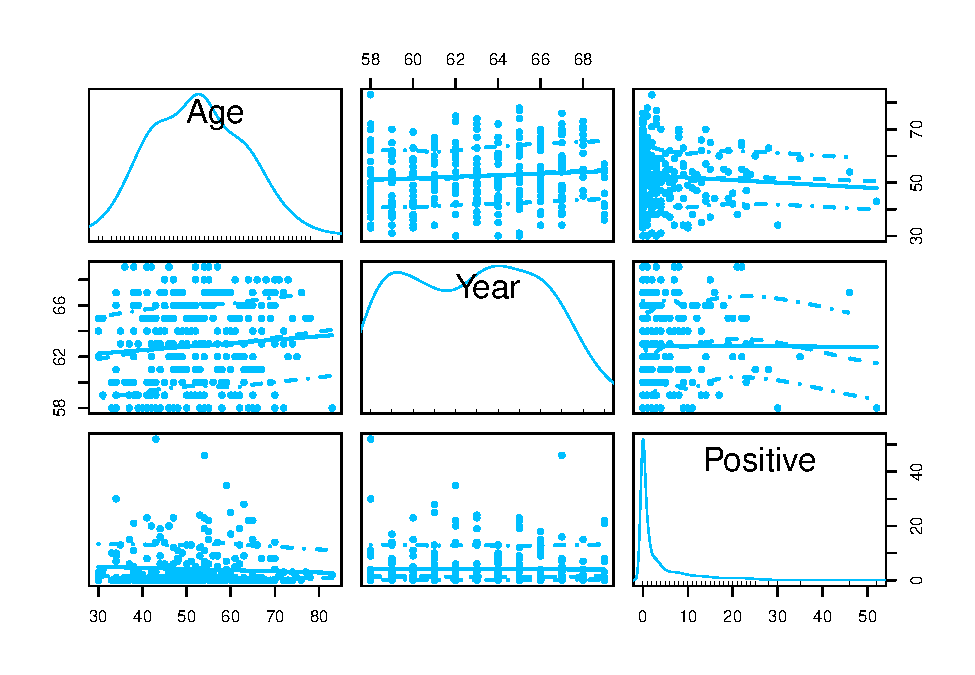
\includegraphics{EDA2_files/figure-latex/unnamed-chunk-28-1} \end{center}

El scatterplot anterior nos muestra mejor la forma de las relaciones
entre variables, vemos que no existe tendencia alguna.

Miramos la distribución de las variables con su clasificación

\begin{Shaded}
\begin{Highlighting}[]
\NormalTok{haberman }\OperatorTok\StringTok{ }
\StringTok{  }\KeywordTok{bind_cols}\NormalTok{(labels) }\OperatorTok\StringTok{ }
\StringTok{  }\KeywordTok{ggplot}\NormalTok{(}\KeywordTok{aes}\NormalTok{(}\DataTypeTok{x=}\NormalTok{Age, }\DataTypeTok{y=}\NormalTok{Year, }\DataTypeTok{color=}\NormalTok{Survival)) }\OperatorTok{+}
\StringTok{    }\KeywordTok{geom_point}\NormalTok{() }\OperatorTok{+}
\StringTok{    }\KeywordTok{labs}\NormalTok{(}\DataTypeTok{title=}\StringTok{"Plot Age-Year con su Survival"}\NormalTok{) }\OperatorTok{+}
\StringTok{    }\KeywordTok{theme_light}\NormalTok{()}
\end{Highlighting}
\end{Shaded}

\begin{center}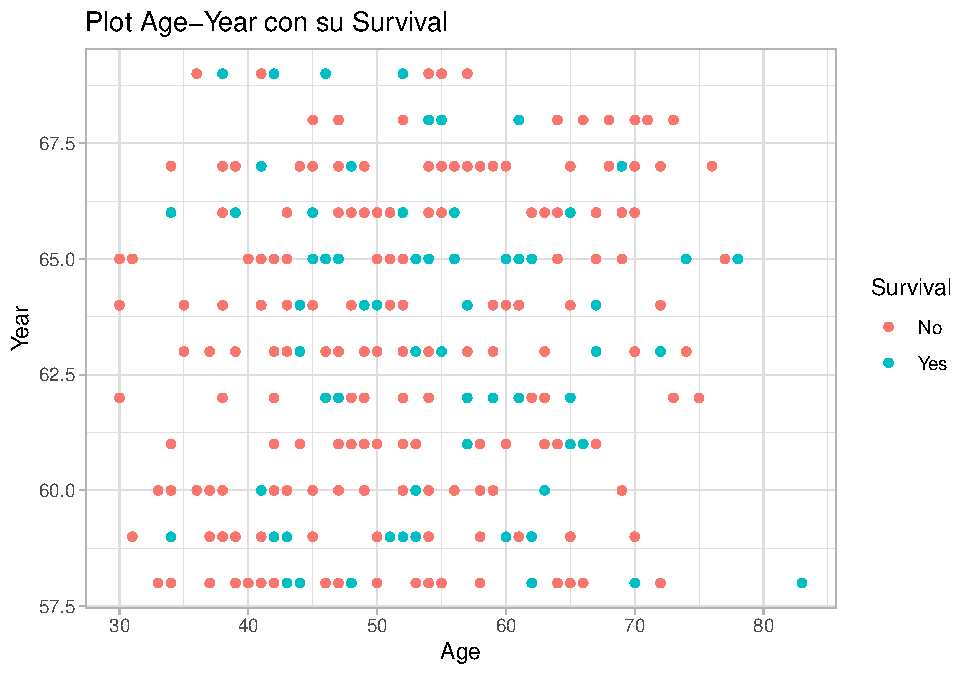
\includegraphics{EDA2_files/figure-latex/unnamed-chunk-29-1} \end{center}

\begin{Shaded}
\begin{Highlighting}[]
\NormalTok{haberman }\OperatorTok\StringTok{ }
\StringTok{  }\KeywordTok{bind_cols}\NormalTok{(labels) }\OperatorTok\StringTok{ }
\StringTok{  }\KeywordTok{ggplot}\NormalTok{(}\KeywordTok{aes}\NormalTok{(}\DataTypeTok{y=}\NormalTok{Age, }\DataTypeTok{x=}\NormalTok{Positive, }\DataTypeTok{color=}\NormalTok{Survival)) }\OperatorTok{+}
\StringTok{    }\KeywordTok{geom_point}\NormalTok{() }\OperatorTok{+}
\StringTok{    }\KeywordTok{labs}\NormalTok{(}\DataTypeTok{title=}\StringTok{"Plot Age-Year con su Survival"}\NormalTok{) }\OperatorTok{+}
\StringTok{    }\KeywordTok{theme_light}\NormalTok{()}
\end{Highlighting}
\end{Shaded}

\begin{center}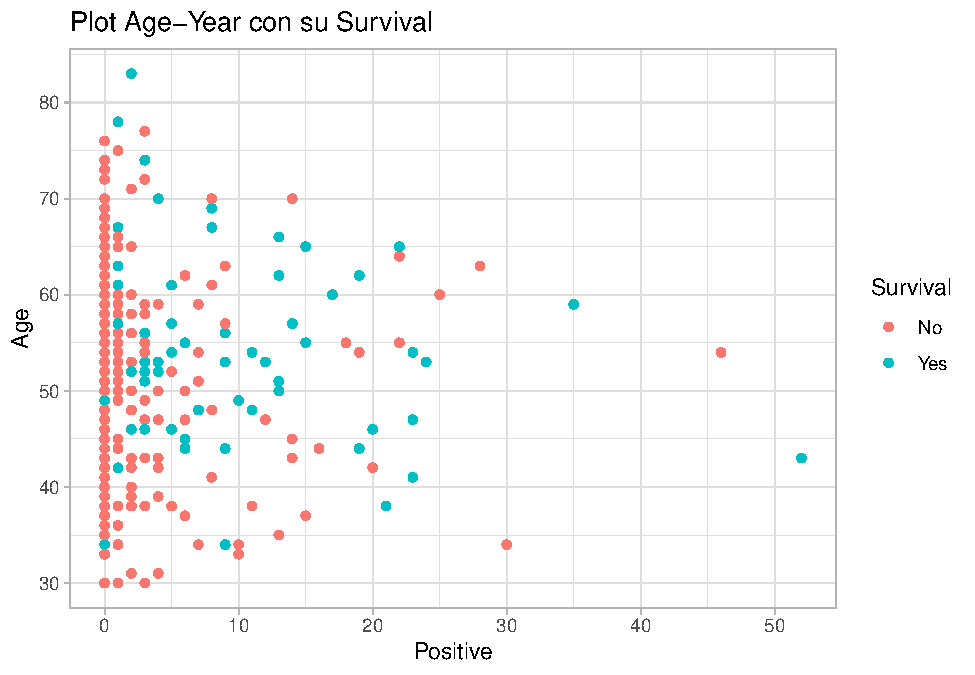
\includegraphics{EDA2_files/figure-latex/unnamed-chunk-29-2} \end{center}

\begin{Shaded}
\begin{Highlighting}[]
\NormalTok{haberman }\OperatorTok\StringTok{ }
\StringTok{  }\KeywordTok{bind_cols}\NormalTok{(labels) }\OperatorTok\StringTok{ }
\StringTok{  }\KeywordTok{ggplot}\NormalTok{(}\KeywordTok{aes}\NormalTok{(}\DataTypeTok{x=}\NormalTok{Year, }\DataTypeTok{y=}\NormalTok{Positive, }\DataTypeTok{color=}\NormalTok{Survival)) }\OperatorTok{+}
\StringTok{    }\KeywordTok{geom_point}\NormalTok{() }\OperatorTok{+}
\StringTok{    }\KeywordTok{labs}\NormalTok{(}\DataTypeTok{title=}\StringTok{"Plot Age-Year con su Survival"}\NormalTok{) }\OperatorTok{+}
\StringTok{    }\KeywordTok{theme_light}\NormalTok{()}
\end{Highlighting}
\end{Shaded}

\begin{center}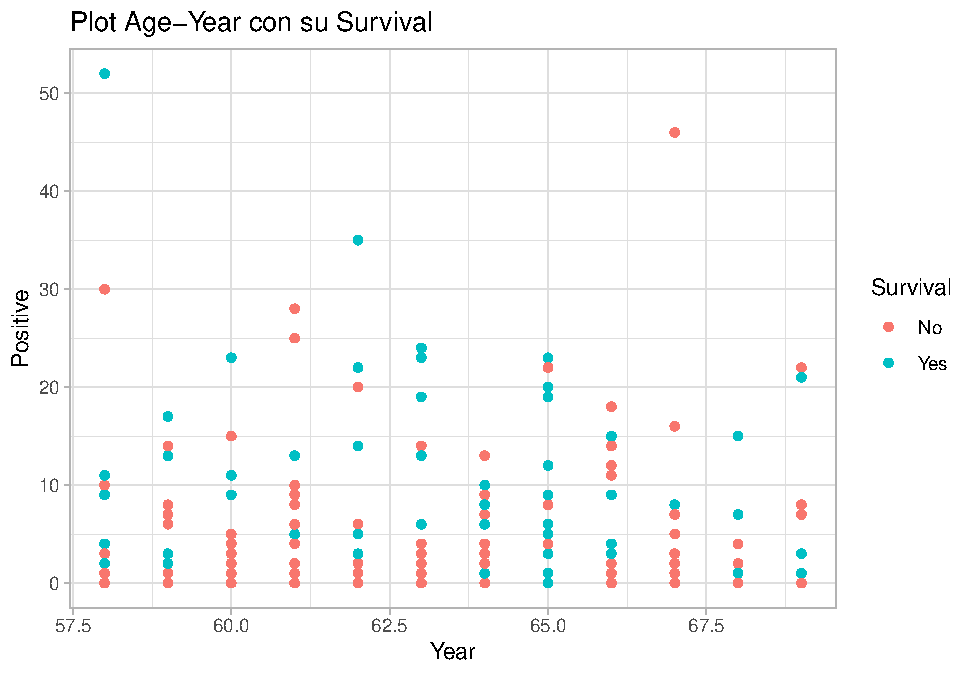
\includegraphics{EDA2_files/figure-latex/unnamed-chunk-29-3} \end{center}

No se aprecia ninguna relación visual que nos ayude a clasificar el
Survival.

\begin{center}\rule{0.5\linewidth}{0.5pt}\end{center}

\hypertarget{tratamiento-de-variables-y-ordenaciones}{%
\subsubsection{Tratamiento de variables y
ordenaciones}\label{tratamiento-de-variables-y-ordenaciones}}

Volvemos a mostrar la cabecera de los datos:

\begin{Shaded}
\begin{Highlighting}[]
\KeywordTok{head}\NormalTok{(haberman)}
\end{Highlighting}
\end{Shaded}

\begin{tabular}{r|r|r}
\hline
Age & Year & Positive\\
\hline
38 & 59 & 2\\
\hline
39 & 63 & 4\\
\hline
49 & 62 & 1\\
\hline
53 & 60 & 2\\
\hline
47 & 68 & 4\\
\hline
56 & 67 & 0\\
\hline
\end{tabular}

Para este dataset contamos con tres clasificadores con información de
distinto tipo y bien organizada, por lo que no necesitamos hacer ningún
tipo de ordenación/tratamiento. No existe ninguna relación entre
variables sobre la información que codifican (en el sentido de que
podrían agruparse).

La variable Year solo indica las dos últimas cifras del año de
operación, pero como todas las instancias son del mismo siglo nos
resulta más conveniente tenerla así

\begin{center}\rule{0.5\linewidth}{0.5pt}\end{center}

\hypertarget{resoluciuxf3n-de-hipuxf3tesis}{%
\paragraph{Resolución de
hipótesis}\label{resoluciuxf3n-de-hipuxf3tesis}}

Nos habíamos planteado las siguientes hipótesis

\begin{itemize}
\tightlist
\item
  H.1: Habrá menor ratio de supervivencia cuanto mayor sea el número de
  nodos positivos encontrados: Por los razonamientos explicados en la
  introducción del problema.
\end{itemize}

\begin{Shaded}
\begin{Highlighting}[]
\NormalTok{haberman }\OperatorTok\StringTok{ }
\StringTok{  }\KeywordTok{bind_cols}\NormalTok{(labels) }\OperatorTok\StringTok{ }
\StringTok{  }\KeywordTok{ggplot}\NormalTok{(}\KeywordTok{aes}\NormalTok{(}\DataTypeTok{x=}\NormalTok{Positive, }\DataTypeTok{fill=}\NormalTok{Survival)) }\OperatorTok{+}
\StringTok{    }\KeywordTok{geom_bar}\NormalTok{() }\OperatorTok{+}
\StringTok{    }\KeywordTok{facet_wrap}\NormalTok{(}\OperatorTok{~}\StringTok{ }\NormalTok{Survival) }\OperatorTok{+}
\StringTok{    }\KeywordTok{theme_light}\NormalTok{()}
\end{Highlighting}
\end{Shaded}

\begin{center}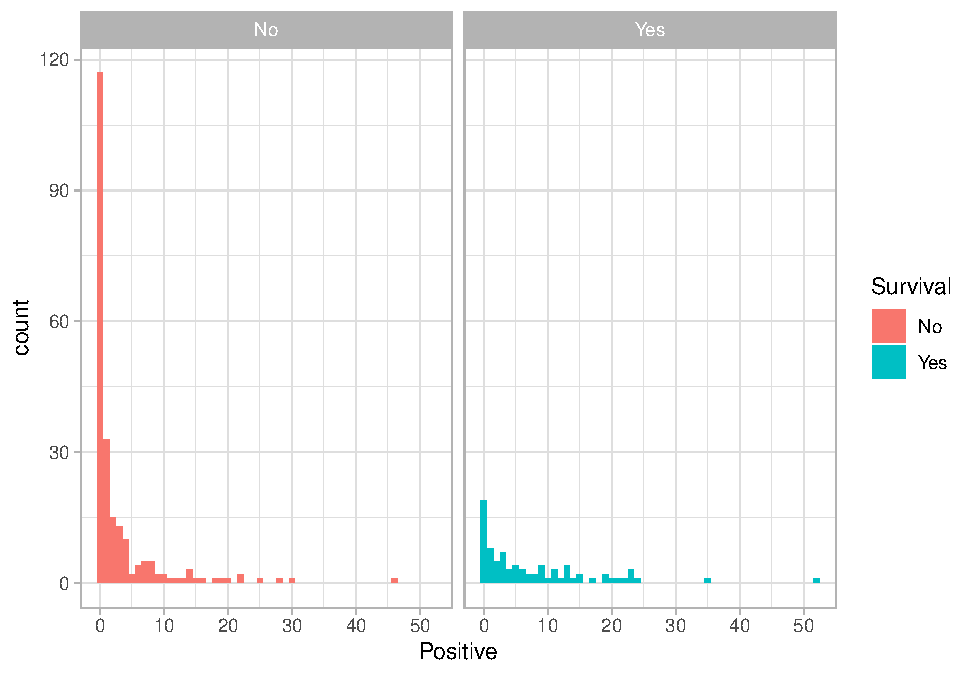
\includegraphics{EDA2_files/figure-latex/unnamed-chunk-31-1} \end{center}

\begin{Shaded}
\begin{Highlighting}[]
\NormalTok{haberman }\OperatorTok\StringTok{ }
\StringTok{  }\KeywordTok{bind_cols}\NormalTok{(labels) }\OperatorTok\StringTok{ }
\StringTok{  }\KeywordTok{filter}\NormalTok{(Positive}\OperatorTok{>}\DecValTok{10}\NormalTok{) }\OperatorTok
\StringTok{  }\KeywordTok{summarise}\NormalTok{(Survival) }\OperatorTok\StringTok{ }
\StringTok{  }\KeywordTok{table}\NormalTok{()}
\end{Highlighting}
\end{Shaded}

\begin{verbatim}
.
 No Yes 
 17  23 
\end{verbatim}

Vemos que la hipótesis no es cierta

\begin{itemize}
\tightlist
\item
  H.2: Habrá mayor ratio de supervivencia cuanto más joven sea el
  paciente.
\end{itemize}

\begin{Shaded}
\begin{Highlighting}[]
\NormalTok{haberman }\OperatorTok\StringTok{ }
\StringTok{  }\KeywordTok{bind_cols}\NormalTok{(labels) }\OperatorTok\StringTok{ }
\StringTok{  }\KeywordTok{ggplot}\NormalTok{(}\KeywordTok{aes}\NormalTok{(}\DataTypeTok{x=}\NormalTok{Age, }\DataTypeTok{fill=}\NormalTok{Survival)) }\OperatorTok{+}
\StringTok{    }\KeywordTok{geom_bar}\NormalTok{() }\OperatorTok{+}
\StringTok{    }\KeywordTok{facet_wrap}\NormalTok{(}\OperatorTok{~}\StringTok{ }\NormalTok{Survival) }\OperatorTok{+}
\StringTok{    }\KeywordTok{theme_light}\NormalTok{()}
\end{Highlighting}
\end{Shaded}

\begin{center}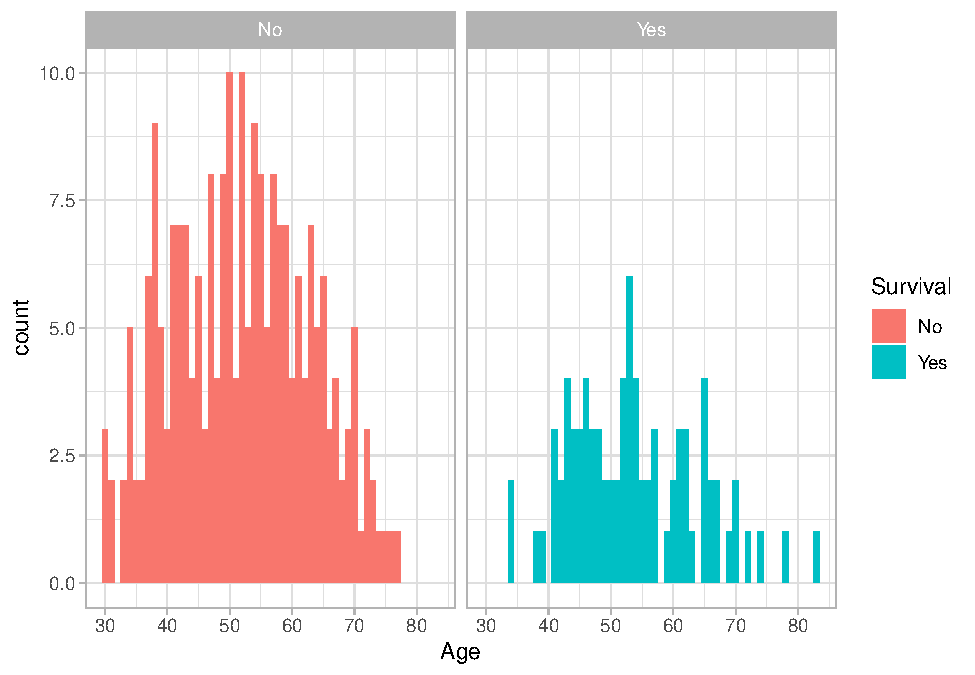
\includegraphics{EDA2_files/figure-latex/unnamed-chunk-33-1} \end{center}

Si miramos los pacientes \textless40

\begin{Shaded}
\begin{Highlighting}[]
\NormalTok{haberman }\OperatorTok\StringTok{ }
\StringTok{  }\KeywordTok{bind_cols}\NormalTok{(labels) }\OperatorTok\StringTok{ }
\StringTok{  }\KeywordTok{filter}\NormalTok{(Age}\OperatorTok{<}\DecValTok{40}\NormalTok{) }\OperatorTok
\StringTok{  }\KeywordTok{summarise}\NormalTok{(Survival) }\OperatorTok\StringTok{ }
\StringTok{  }\KeywordTok{table}\NormalTok{()}
\end{Highlighting}
\end{Shaded}

\begin{verbatim}
.
 No Yes 
 36   4 
\end{verbatim}

Nos sale todo lo contrario.

\begin{itemize}
\tightlist
\item
  H.3: El rango de Year es pequeño. La influencia de esta variable
  creemos que podría darse solo si durante ese período se hubieran
  descubierto técnicas mejores de cirugía. Este razonamiento va
  orientado de cara a la población y no a la muestra. Puesto que
  contamos con datos de un solo hospital durante pocos años, es posible
  que el equipo de cirugía hubiera sido el mismo para la mayoría de
  pacientes.
\end{itemize}

\begin{Shaded}
\begin{Highlighting}[]
\NormalTok{haberman }\OperatorTok\StringTok{ }
\StringTok{  }\KeywordTok{bind_cols}\NormalTok{(labels) }\OperatorTok\StringTok{ }
\StringTok{  }\KeywordTok{ggplot}\NormalTok{(}\KeywordTok{aes}\NormalTok{(}\DataTypeTok{x=}\NormalTok{Year, }\DataTypeTok{fill=}\NormalTok{Survival)) }\OperatorTok{+}
\StringTok{    }\KeywordTok{geom_bar}\NormalTok{() }\OperatorTok{+}
\StringTok{    }\KeywordTok{labs}\NormalTok{(}\DataTypeTok{title=}\StringTok{"Survival en base a Year"}\NormalTok{) }\OperatorTok{+}
\StringTok{    }\KeywordTok{theme_light}\NormalTok{()}
\end{Highlighting}
\end{Shaded}

\begin{center}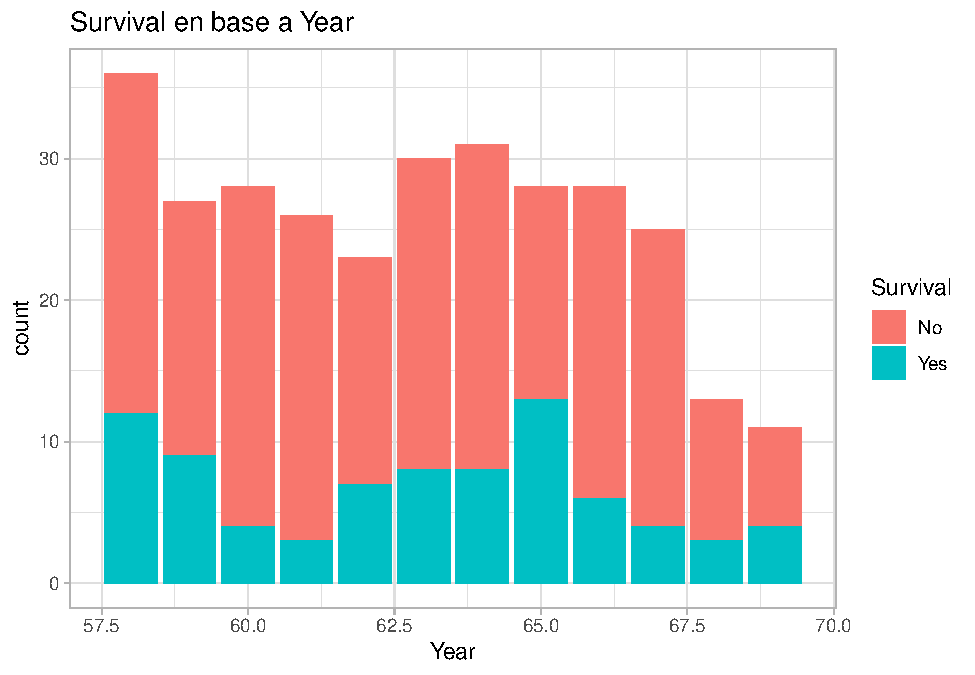
\includegraphics{EDA2_files/figure-latex/unnamed-chunk-35-1} \end{center}

Decrementa el número de datos en años superiores, aunque las
proporciones parecen aumentar. Lo mostramos:

\begin{Shaded}
\begin{Highlighting}[]
\NormalTok{haberman }\OperatorTok\StringTok{ }
\StringTok{  }\KeywordTok{bind_cols}\NormalTok{(labels) }\OperatorTok\StringTok{ }
\StringTok{  }\KeywordTok{ggplot}\NormalTok{(}\KeywordTok{aes}\NormalTok{(}\DataTypeTok{x=}\NormalTok{Year, }\DataTypeTok{fill=}\NormalTok{Survival)) }\OperatorTok{+}
\StringTok{    }\KeywordTok{geom_bar}\NormalTok{(}\DataTypeTok{position=}\StringTok{"fill"}\NormalTok{) }\OperatorTok{+}
\StringTok{    }\KeywordTok{labs}\NormalTok{(}\DataTypeTok{title=}\StringTok{"Proporciones Surival en base a Year"}\NormalTok{) }\OperatorTok{+}
\StringTok{    }\KeywordTok{theme_light}\NormalTok{()}
\end{Highlighting}
\end{Shaded}

\begin{center}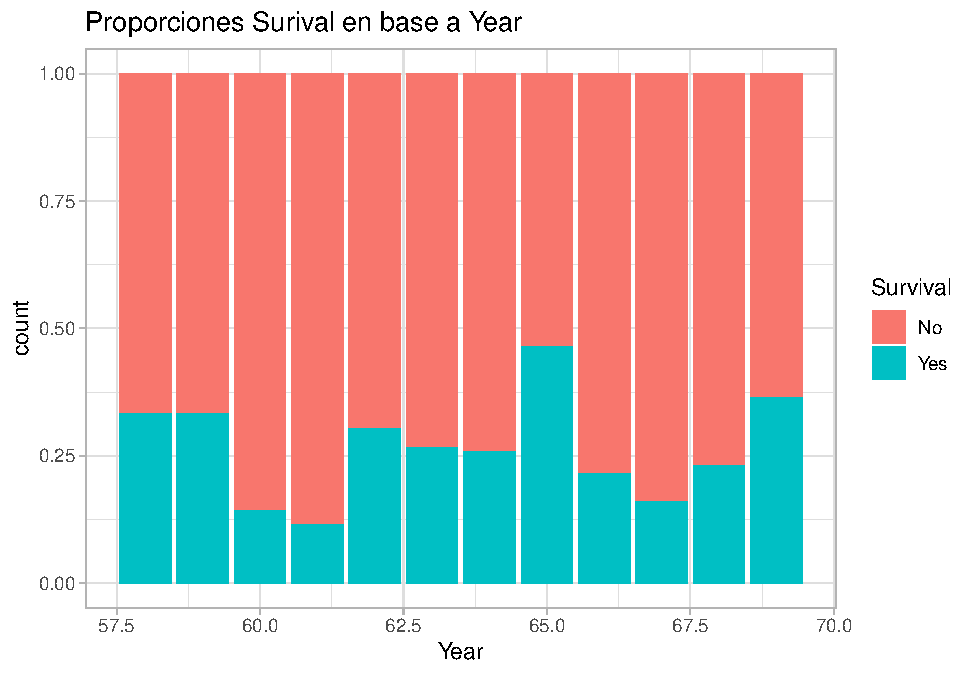
\includegraphics{EDA2_files/figure-latex/unnamed-chunk-36-1} \end{center}

A excepción de algunos años, la porporción es bastante similar con los
datos que tenemos, por lo que no podemos confirmar la hipótesis.

\begin{itemize}
\tightlist
\item
  H.4: Podría haber relación entre la edad y el número de positivos,
  posiblemente indicando lo tardío que se descubre el cáncer.
\end{itemize}

\begin{Shaded}
\begin{Highlighting}[]
\NormalTok{haberman }\OperatorTok\StringTok{ }
\StringTok{  }\KeywordTok{bind_cols}\NormalTok{(labels) }\OperatorTok\StringTok{ }
\StringTok{  }\KeywordTok{ggplot}\NormalTok{(}\KeywordTok{aes}\NormalTok{(}\DataTypeTok{x=}\NormalTok{Age, }\DataTypeTok{y=}\NormalTok{Positive, }\DataTypeTok{color=}\NormalTok{Survival)) }\OperatorTok{+}
\StringTok{    }\KeywordTok{geom_point}\NormalTok{() }\OperatorTok{+}
\StringTok{    }\KeywordTok{labs}\NormalTok{(}\DataTypeTok{title=}\StringTok{"Plot Age-Positive con su Survival"}\NormalTok{) }\OperatorTok{+}
\StringTok{    }\KeywordTok{theme_light}\NormalTok{()}
\end{Highlighting}
\end{Shaded}

\begin{center}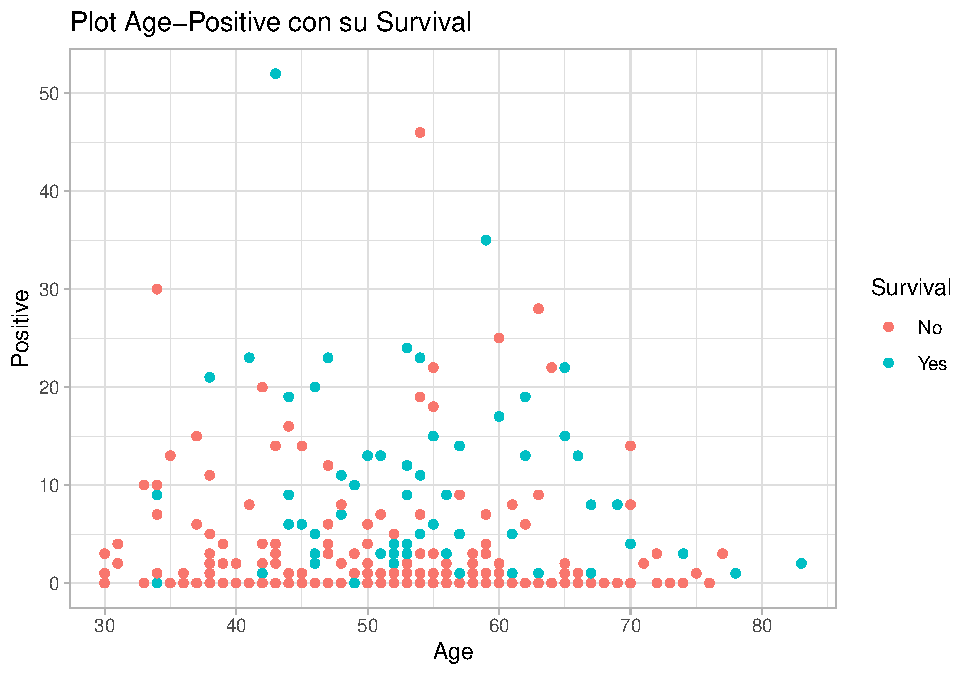
\includegraphics{EDA2_files/figure-latex/unnamed-chunk-37-1} \end{center}

\begin{center}\rule{0.5\linewidth}{0.5pt}\end{center}

\hypertarget{conclusiones}{%
\paragraph{Conclusiones}\label{conclusiones}}

En resumen concluímos diciendo que tenemos un dataset con pocas
variables, pero con ninguna correlación entre ellas, lo que nos favorece
en el problema de clasificación que nos atañe. También hemos visto
ausencia de normalidad en los clasificadores (PONER CONSECUENCIAS DE
ESTO) \ldots{}

Además, contamos con más instancias de no supervivientes, algo que
probablemente no nos resulte favorable para regresión logística y LDA
(SEGURO?)

Únicamente hemos preprocesado los datos aplicando una estandarización,
preparando el dataset a los algoritmos que se van a utilizar.

\end{document}
